\chapter{Swiss Terrain 3D}
\label{chap_swiss_terrain_3d}
Kapitel \ref{chap_datengrundlage} behandelte die Datengrundlage für die Terrainvisualisierung. In Kapitel \ref{chap_technologien} wurden Programme und Frameworks zur Erstellung von 3D-Visualisierungen thematisiert. Die technisch notwendigen Grundlagen zur Grafikprogrammierung wurden im Rahmen von Kapitel \ref{chap_render_pipelines} erläutert. Kapitel \ref{chap_algorithmen} befasste sich mit gängigen Datenstrukturen und Algorithmen. Aufbauend auf diesem Vorwissen geht es in diesem Kapitel nun um die eigentliche Implementierung der Terrainvisualisierung.

\section{Technologie und Anforderungen}
\label{technologie_anforderungen}
Bevor eine Visualisierung implementiert werden kann, müssen sowohl die Anforderungen als auch die hierfür verwendete Technologie festgelegt werden. Eine echtzeitfähige 3D-Visualisierung ist vereinfacht ausgedrückt eine Abfolge von Bildern, welche von der Grafikkarte gezeichnet werden. Diese Bilder werden abhängig von verschiedenen Parametern wie dem Blickwinkel der Kamera, den zugrundeliegenden Daten und den Nutzereingaben generiert. Werden die Bilder schnell genug hintereinander gezeichnet, entsteht eine echtzeitfähige Visualisierung. Damit eine Visualisierung als Echtzeit bezeichnet werden kann, muss die Visualisierung mit mindestens 30 Bildern pro Sekunde (FPS) gezeichnet werden. Moderne Monitore besitzen jedoch Bildwiederholraten, welche weit über 30 FPS gehen. Bildwiederholraten von 60 FPS bis zu 140 FPS sind heute keine Seltenheit mehr. Abgesehen von der Bildwiederholrate spielt auch die Auflösung eine wichtige Rolle. Je höher die Auflösung, desto detailgetreuer lässt sich die Visualisierung darstellen. Sowohl für eine hohe Auflösung wie auch Bildwiederholrate benötigt es eine entsprechend leistungsfähige Grafikkarte, was wiederum Einfluss auf die erreichbare Zielgruppe hat. Die vorliegende Masterarbeit geht hier deshalb einen Mittelweg und legt folgende Mindestanforderungen an die Visualisierung fest. \textit{Die Visualisierung soll mit mindestens 60 Bildern pro Sekunde bei einer Auflösung von 2k laufen}.

Nebst den technischen Anforderungen stellt sich auch die Frage, welche Plattformen unterstützt werden sollen. Heutzutage sind auf den meisten Betriebssystemen sowie mobilen Endgeräten bereits Browser vorinstalliert. Browserbasierte Anwendungen haben zudem den Vorteil, dass keinerlei Installationsaufwand seitens der Nutzer anfällt. Um eine möglichst breite Zielgruppe ohne anfallenden Installationsaufwand abzudecken, hat sich der Autor daher für eine webbasierte Implementierung entschieden. 

Wie in Kapitel \ref{chap_technologien} thematisiert, unterstützen moderne Engines wie Unity, Unreal und Godot das Erstellen von browserbasierten Anwendungen. Die primäre Hauptzielgruppe dieser Engines sind jedoch nach wie vor native Anwendungen und Betriebssysteme. Zudem fallen bei kommerziellen Engines wie Unity und Unreal entsprechende Lizenzgebühren an. Obwohl Engines diverse Programme und Editoren mitbringen, welche das Erstellen von 3D Anwendungen erleichtern, muss der Umgang mit diesen Werkzeugen zuerst erlernt werden. Zudem sind Engines bei auftauchenden technischen Limitationen aufgrund des eingeschränkten Zugriffs auf den Quellcode nur schwer an die eigenen Bedürfnisse anpassbar. Ferner benötigen Engines wie Unreal entsprechend performante Hardware, um überhaupt genutzt werden zu können. Aufgrund dieser Aspekte hat sich der Autor für ein webbasiertes Framework anstelle einer Engine entschieden. Sowohl Three.js als auch Babylon.js unterstützen hierbei die neuesten Grafikschnittstellen wie WebGL2 und WebGPU. Da das \acrshort{CAVE}-System der FHGR jedoch auf dem Three.js Framework basiert und der Autor bereits entsprechende Vorkenntnisse besitzt, wurde dieses gegenüber Babylon.js präferiert. Three.js hat gegenüber Babylon.js zudem den Vorteil, dass auf eine wesentlich grössere Community und ein breites Spektrum von diversen Beispielapplikationen zurückgegriffen werden kann (siehe Kapitel \ref{chap_technologien}).

\section{Datenvorverarbeitung}
Dem Autor war es wichtig, dass die Datenvorverarbeitung nicht manuell von Hand erfolgen muss. Deswegen wurden alle nachfolgend behandelten Aspekte mithilfe eines Python-Skripts weitestgehend automatisiert und müssen daher nicht manuell durchgeführt werden. Abbildung \ref{fig_data_preprocessing} zeigt die komplette Datenvorverarbeitung auf einen Blick. Nachfolgend wird auf die wichtigsten Teilbereiche genauer eingegangen.
\begin{figure}[H]
    \caption{Übersicht Datenvorverarbeitung (Eigene Darstellung)}
    \includegraphics[width=.15\linewidth]{content/00_assets/uebersicht_datenvorverarbeitung.png}
    \label{fig_data_preprocessing}
\end{figure}

\subsection{Herunterladen der Daten}
Sowohl der swissALTI3D wie auch der swissIMAGE-Datensatz stehen kostenfrei über die swisstopo Webseite zum Download bereit (siehe Abbildung \ref{fig_swisstopo_datenbezug}). Zu Beginn muss der geografische Bereich ausgewählt werden. Dies geschieht über die Auswahl einer Gemeinde, eines Kantons oder über das Definieren eines 2D-Bereichs auf der Karte (siehe Bereich A in Abbildung \ref{fig_swisstopo_datenbezug}). Anschliessend werden das gewünschte Datenformat sowie die entsprechende Auflösung ausgewählt (siehe Bereich B in Abbildung \ref{fig_swisstopo_datenbezug}). Daraufhin kann eine entsprechende CSV-Datei heruntergeladen werden. Die CSV-Datei beinhaltet eine Sammlung von Hyperlinks auf die entsprechenden Datensätze. Ein Datensatz repräsentiert jeweils  einen geografischen Bereich von jeweils einem Quadtratkilometer. Diese Bereiche werden fortlaufend als ``Tiles'' bezeichnet. Damit die Daten nicht einzeln heruntergeladen werden müssen, wurde ein Python-Skript geschrieben, welches die CSV-Datei einliest, die Dateien herunterlädt und in konfigurierbare Ordner abspeichert.
\begin{figure}[H]
    \caption{Herunterladen der swisstopo Daten (Eigene Darstellung)}
    \includegraphics[width=.4\linewidth]{content/00_assets/swisstopo_datenauswahl.png}
    \label{fig_swisstopo_datenbezug}
\end{figure}

Die Links zu den Daten, welche in den CSV-Dateien befinden, erstrecken sich nicht immer über einen kontinuierlichen Bereich. Wählt man beispielsweise die Region Sarganserland auf der swisstopo-Webseite aus und setzt anschliessend die Tiles zu einem Gesamtbild zusammen, wird ersichtlich, dass entsprechende Lücken vorhanden sind (siehe schwarze Bereiche in der Abbildung \ref{fig_swisstopo_daten_luecken}). Da die Daten jedoch entsprechend georeferenziert sind und auf dem LV95-Koordinatensystem basieren, können die fehlenden Bereiche detektiert und entsprechend geschlossen werden (siehe Abbildung \ref{fig_swisstopo_daten_luecken}).

\begin{figure}[H]
    \caption{Lücken in swisstopo-Daten (links) mit automatischer Korrektur (rechts) (Eigene Darstellung)}
    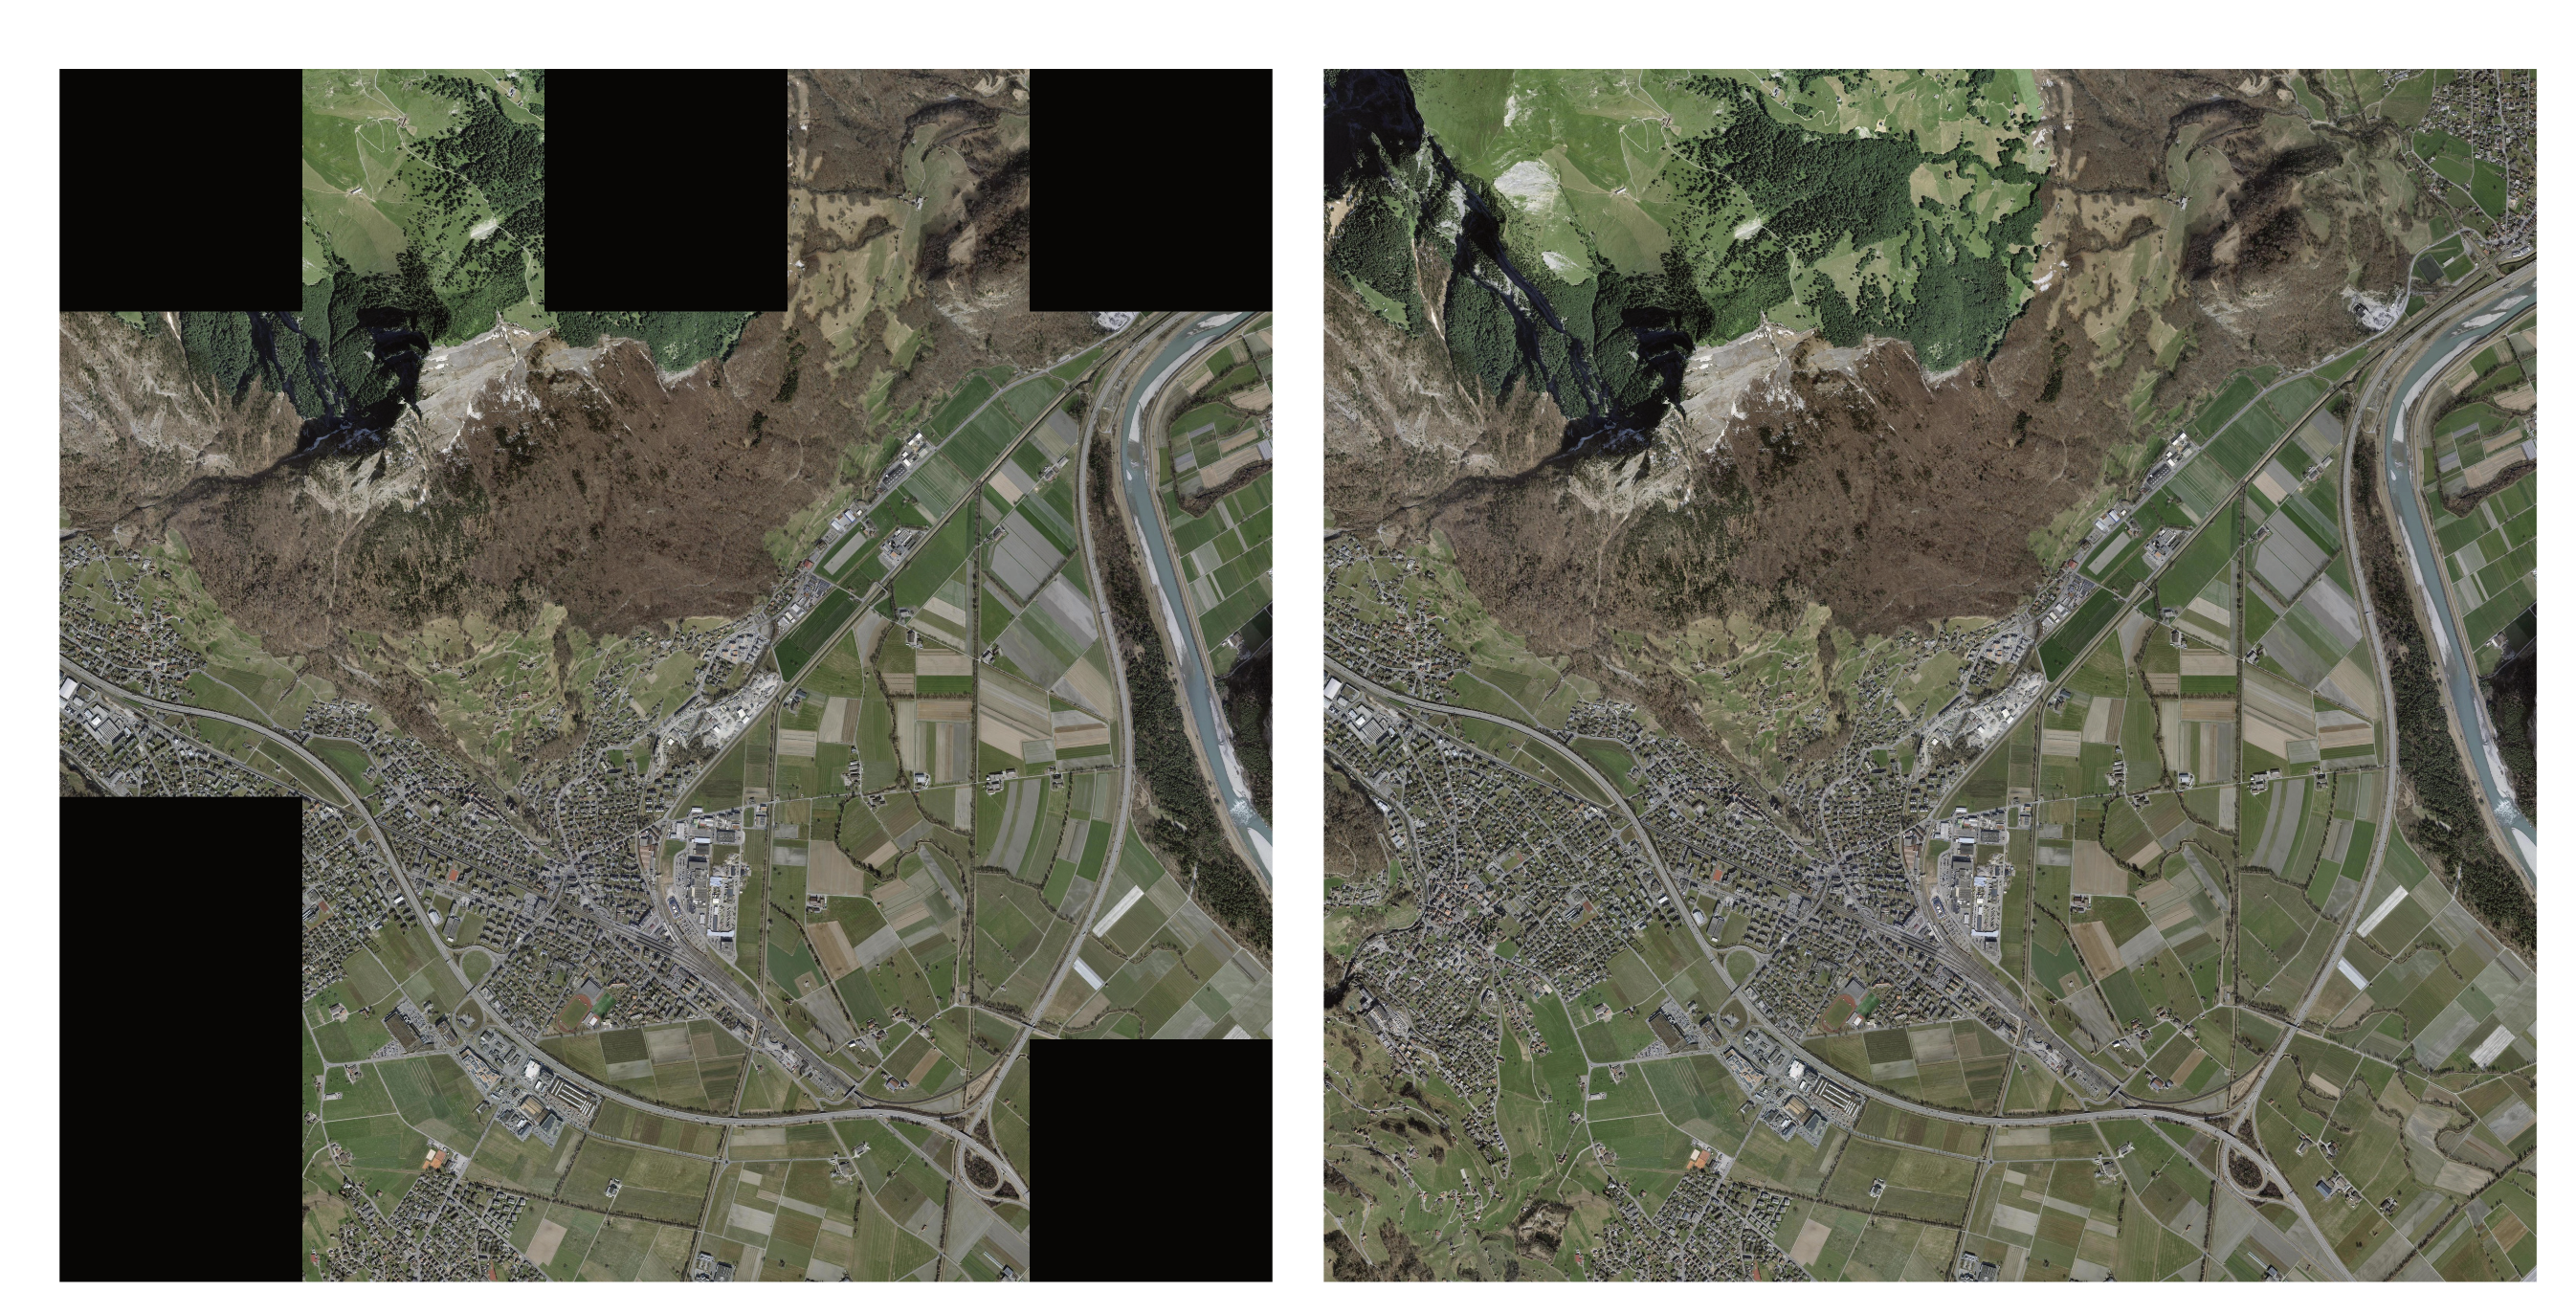
\includegraphics[width=.6\linewidth]{content/00_assets/gesamtbild_mit_luecken.png}
    \label{fig_swisstopo_daten_luecken}
\end{figure}

\subsection{Extrahierung der Höhenwerte und Bilddaten}
Sind die Daten heruntergeladen, müssen sowohl die Bild- als auch die Höhenwerte aus den GeoTIFF-Dateien gelesen und als eigenständige Texturen (Bilder) abgespeichert werden. Die Höhenwerte werden hierbei als Graustufenbild gespeichert. Weisse Farben bedeuten hohe Werte, wohingegen niedrige Höhenwerte mit der Farbe Schwarz dargestellt werden (siehe Abbildung \ref{fig_heightmap_beispiel}). 
\begin{figure}[H]
    \caption{Extrahierte Höhenwerte als Graustufenbild (Eigene Darstellung)}
    \includegraphics[width=.4\linewidth]{content/00_assets/heightmap_beispiel.png}
    \label{fig_heightmap_beispiel}
\end{figure}

Um die Geopositionsdaten nicht zu verlieren, werden diese in den Dateinamen geschrieben. Da die Daten von swisstopo in Form von Tiles zur Verfügung gestellt werden, müssen diese in einem nächsten Schritt zu einem Gesamtbild zusammengesetzt werden. Da die Geoposition anhand des LV95-Koordinatensystems bekannt ist, können diese anhand der Nord- und Ostachsenwerte entsprechend zusammengesetzt werden. Hierbei offenbart sich jedoch das erste Problem mit den Höhenwerten. Jede Kachel besitzt einen eigenen minimalen sowie maximalen Höhenwert. Werden diese zusammengesetzt, so gibt es keine fliessenden Übergänge. Um dieses Problem zu lösen, wurden die Höhenwerte anhand des globalen Minimums und Maximums normalisiert (siehe Abbildung \ref{fig_heightmap_sargans}).
\begin{figure}[H]
    \caption{Zusammengesetztes Graustufenbild von Sargans mit fliessenden (links) und nicht fliessenden (rechts) Übergängen (Eigene Darstellung)}
    \includegraphics[width=.7\linewidth]{content/00_assets/heightmap_sargans.png}
    \label{fig_heightmap_sargans}
\end{figure}

Das Extrahieren der Farbwerte aus dem swissIMAGE-Datensatz ist einfacher, da lediglich die Farbwerte aus den Dateien herausgelesen werden müssen und keine Normalisierung notwendig ist (siehe Abbildung \ref{fig_textur_sargans}). Aufgrund unterschiedlicher Aufnahmezeiträume können jedoch visuelle Diskrepanzen wie im Bereich A (siehe Abbildung \ref{fig_textur_sargans}) entstehen.
\begin{figure}[H]
    \caption{Zusammengesetztes Luftbild von Sargans (Eigene Darstellung)}
    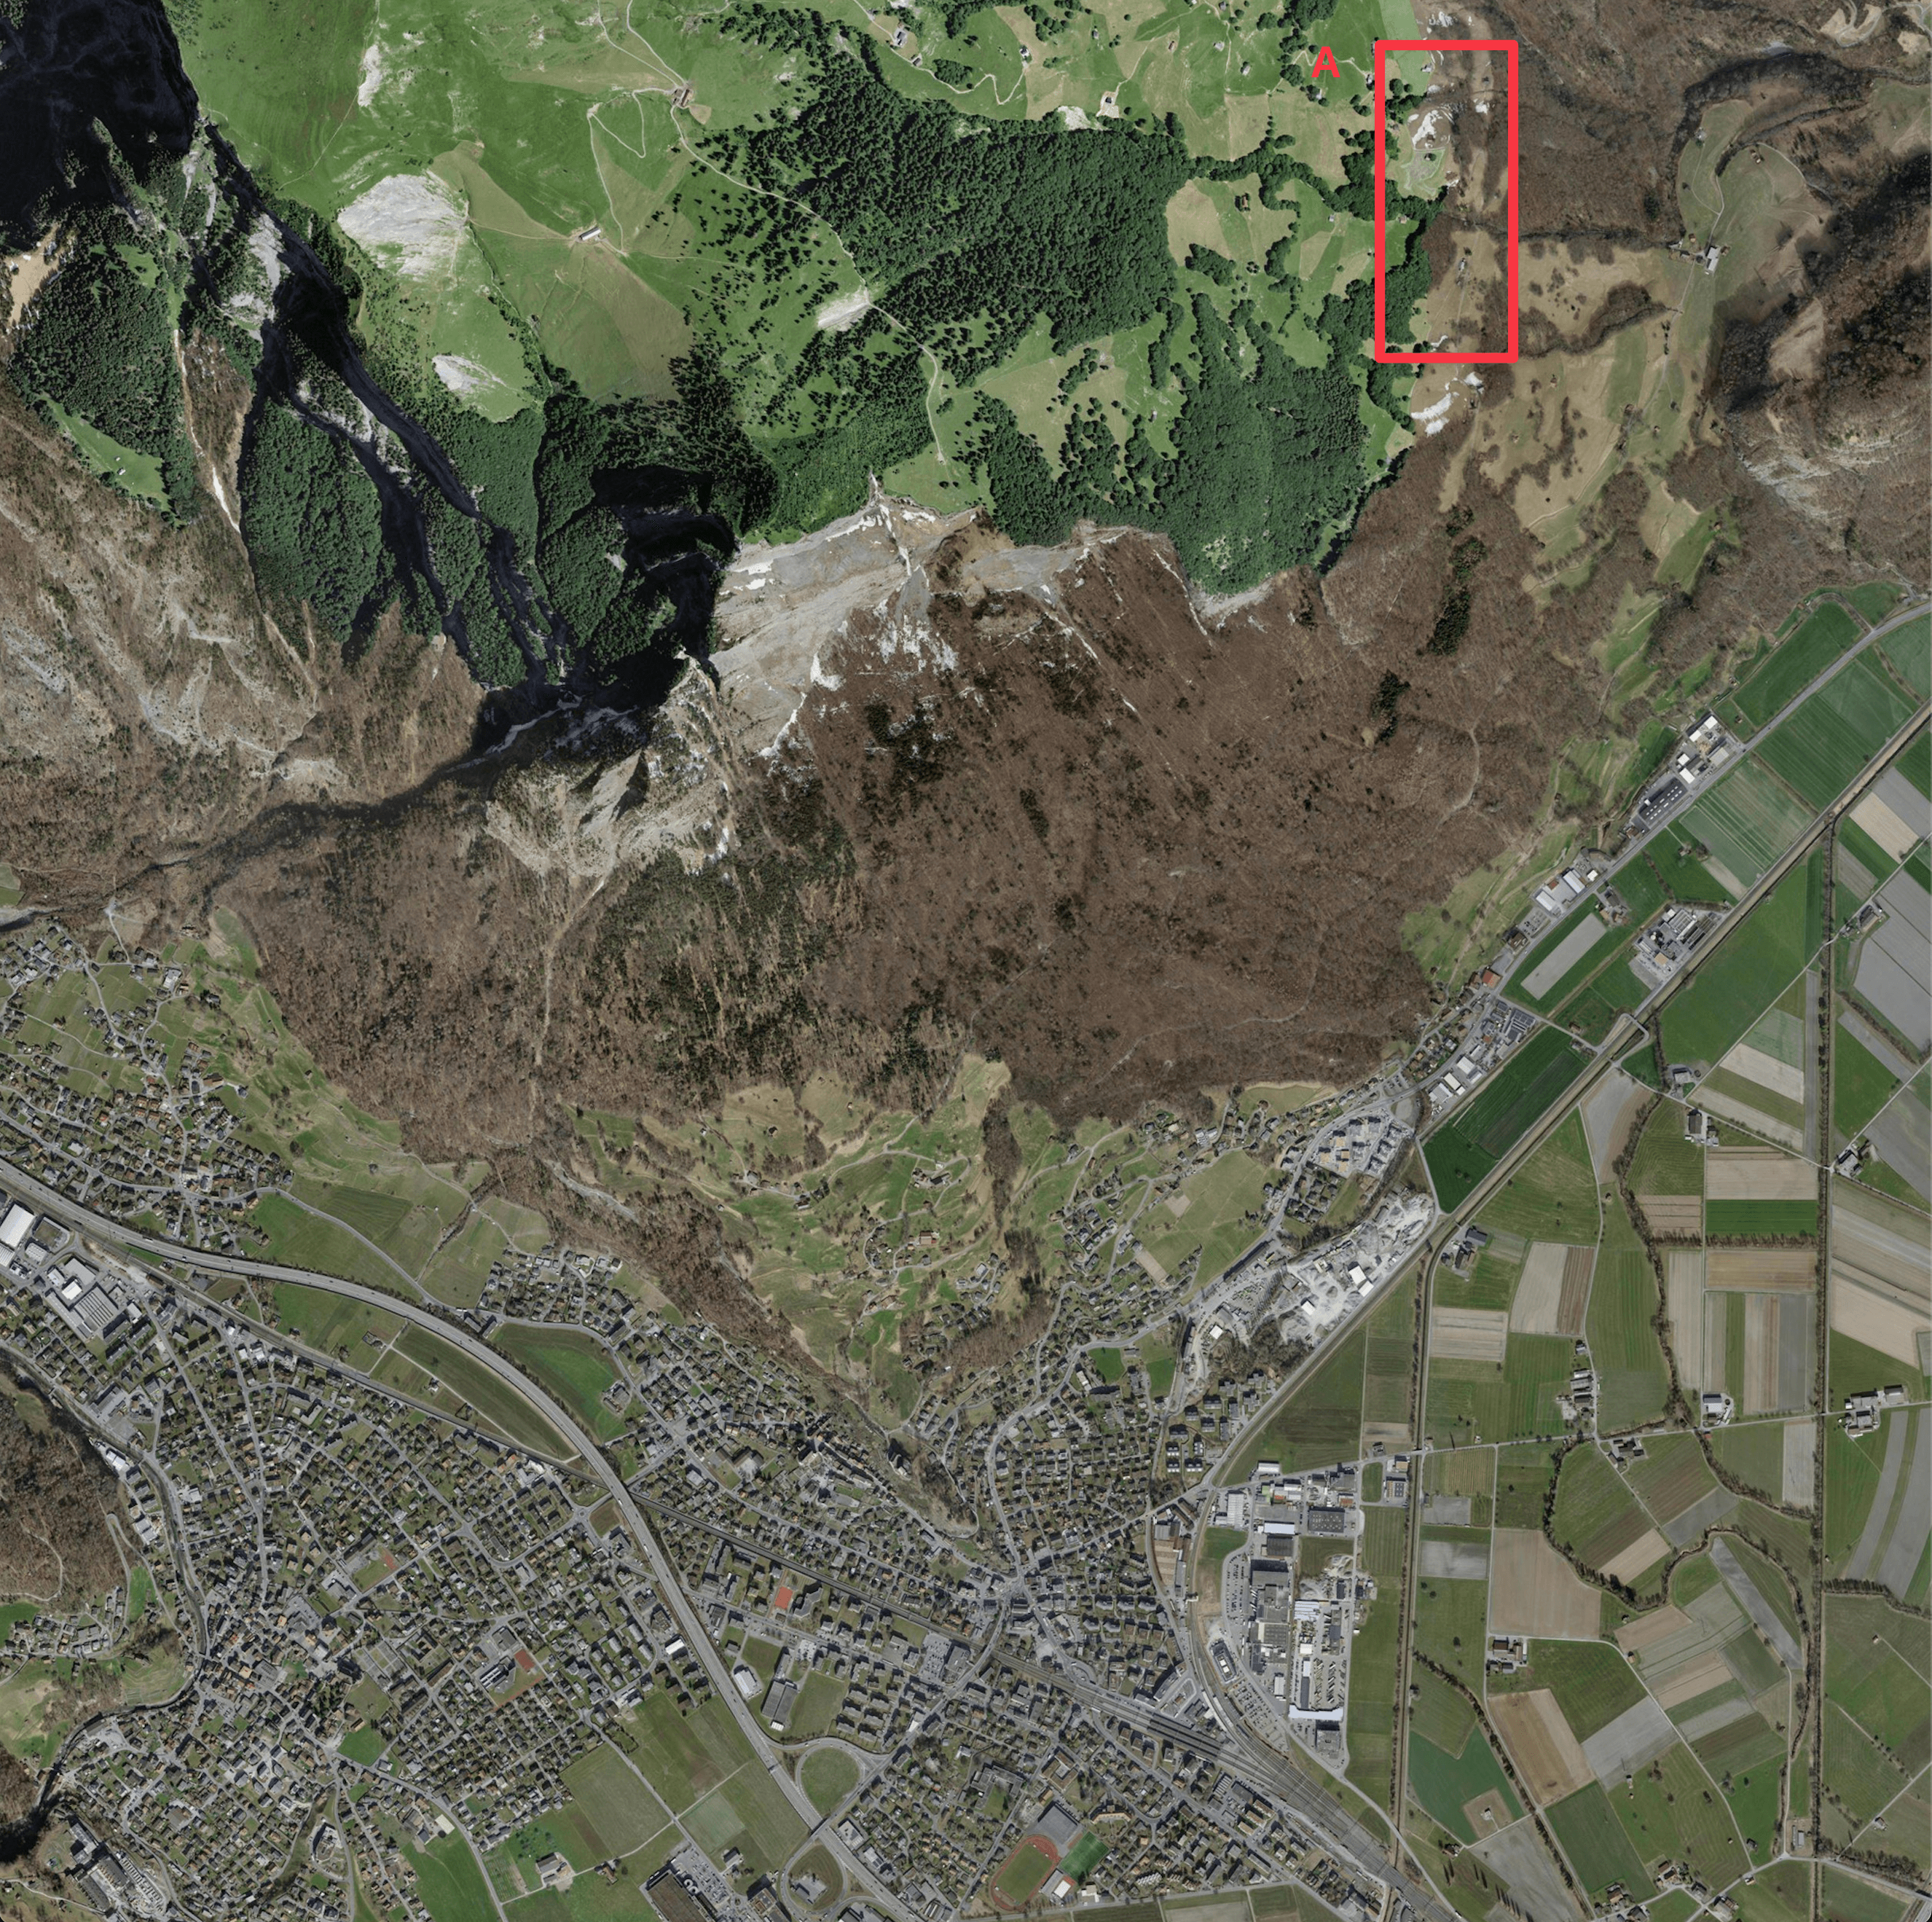
\includegraphics[width=.4\linewidth]{content/00_assets/textur_sargans.png}
    \label{fig_textur_sargans}
\end{figure}

\subsection{Aufteilung in kleinere Bilddateien}
Wie in Kapitel \ref{chap_datengrundlage} thematisiert, benötigen die swisstopo Datensätze je nach Auflösung und Gebiet unterschiedlich viel Festplattenspeicher. Setzt man die einzelnen Luftbilder für den Raum Sargans in der höchsten Auflösung von 10cm pro Bildpunkt zu einem Gesamtbild zusammen, so werden rund 7.5GB Festplattenspeicher benötigt. Sofern nicht lange Ladezeiten in Kauf genommen werden, ist solch eine Grösse für eine Browseranwendung nicht zu empfehlen. Browserbasierte Anwendungen haben gegenüber nativen Applikationen zwar den Vorteil, dass sie von überall aus zugreifbar sind, jedoch müssen hierzu die notwendigen Daten auch auf das Zielsystem des Nutzers heruntergeladen werden. Je nach Internetbandbreite kann dieser Prozess viel Zeit benötigen. Das Herunterladen von grossen Dateien ist daher trotz Konzepten wie Ladebalken keine skalierbare Lösung.

Um dieses Problem zu lösen, werden im Rahmen der Datenvorverarbeitung verschiedene Schritte durchgeführt. Zu Beginn wird das Gesamtbild in kleinere Bilddateien (Tiles) aufgeteilt. Um den Speicherverbrauch zu minimieren und die Ladezeiten zu verkürzen, werden diese anschliessend mithilfe eines Downsampling-Algorithmus herunterskaliert. Die Erstellung der Tiles anhand des Quadtree Algorithmus. Hierzu werden Tiles in unterschiedlichen Auflösungen (LOD) erstellt. Die Auflösung entspricht hierbei der Baumtiefe. Für die erste Auflösung (LOD 1) wird das Gesamtbild in 4 (4$^1$) Tiles aufgeteilt. Für die zweite Auflösung sind es hingegen 16 (4$^2$) Tiles und so weiter. Abbildung \ref{fig_textur_teilbilder_quadtree} zeigt, wie ein Gesamtbild in Tiles mit unterschiedlichen Auflösungen aufgeteilt wird.
\begin{figure}[H]
    \caption{Aufteilung in Tiles mit unterschiedlichen Auflösungen (Eigene Darstellung)}
    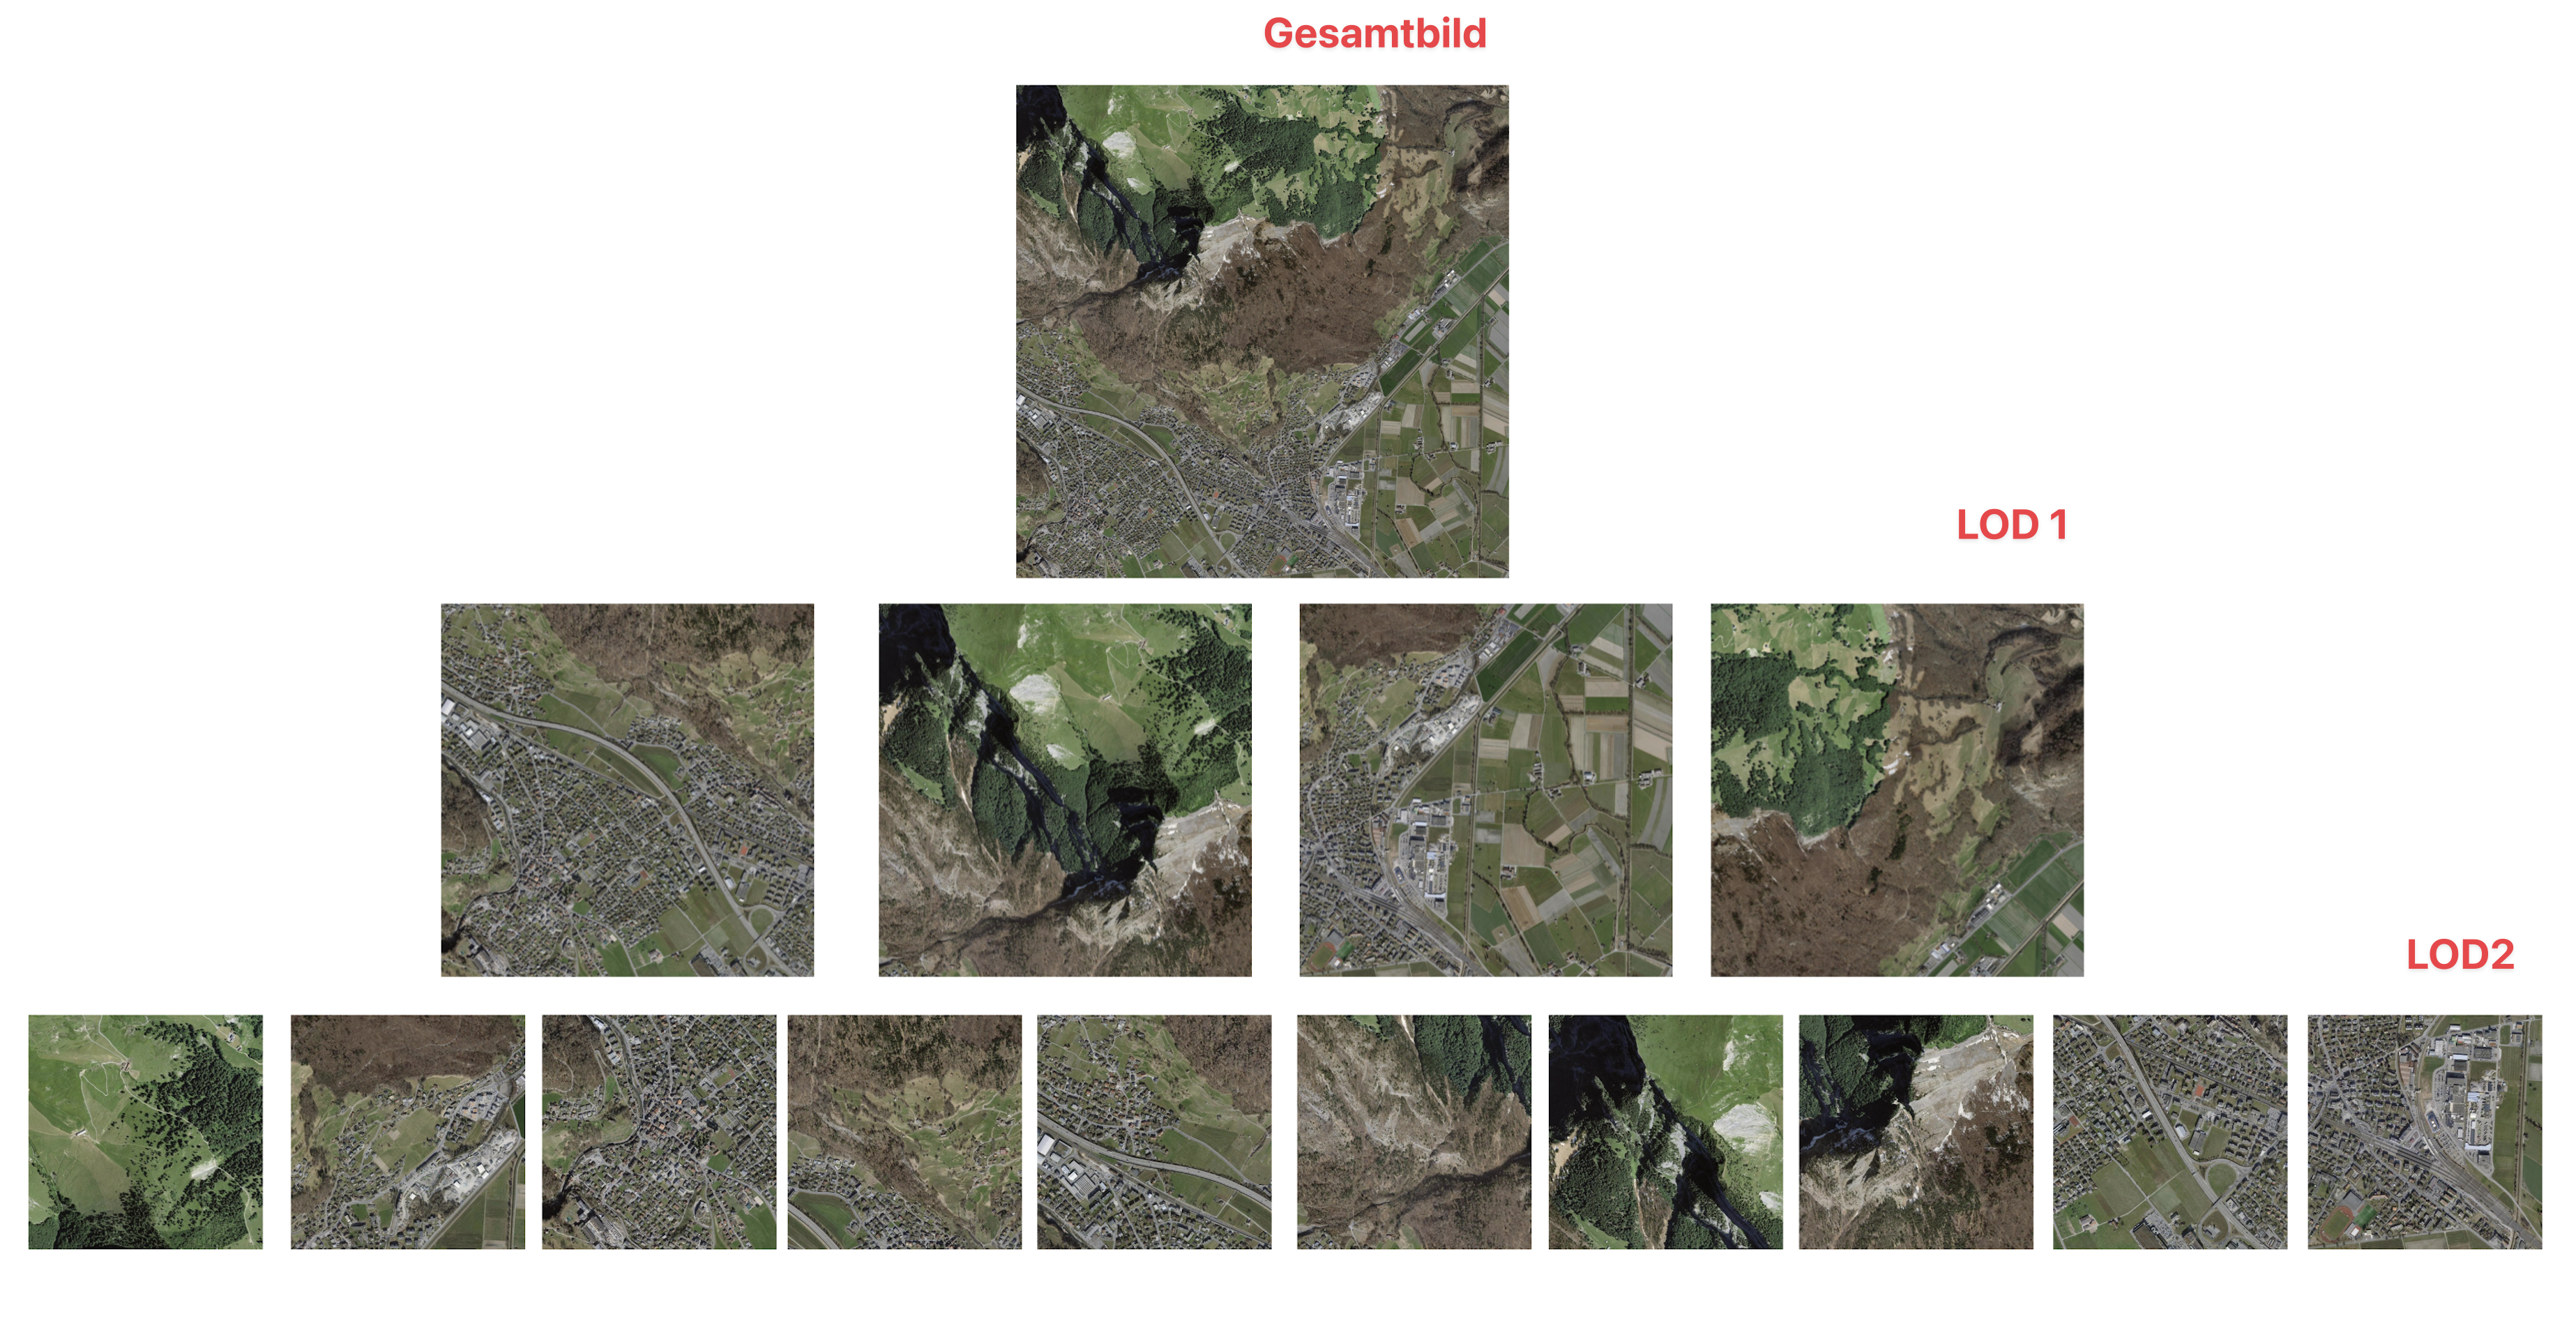
\includegraphics[width=1.0\linewidth]{content/00_assets/zerlegung_in_teilbilder.png}
    \label{fig_textur_teilbilder_quadtree}
\end{figure}

\subsection{Ermittlung des quadratischen Bildausschnitts}
Grafikkarten bevorzugen aus Performanzgründen Texturen mit einer quadratischen Auflösung (500px auf 500px etc.). Jedoch erstrecken sich die swisstopo-Daten je nach Region und Ausschnitt, nicht immer über einen quadratischen Bereich. Um dies zu gewährleisten, wird das Gesamtbild zusätzlich auf einen quadratischen Bildausschnitt beschränkt (siehe Abbildung \ref{fig_begrenzung_bildausschnitt}). 
\begin{figure}[H]
    \caption{Begrenzung Bildausschnitt (Eigene Darstellung)}
    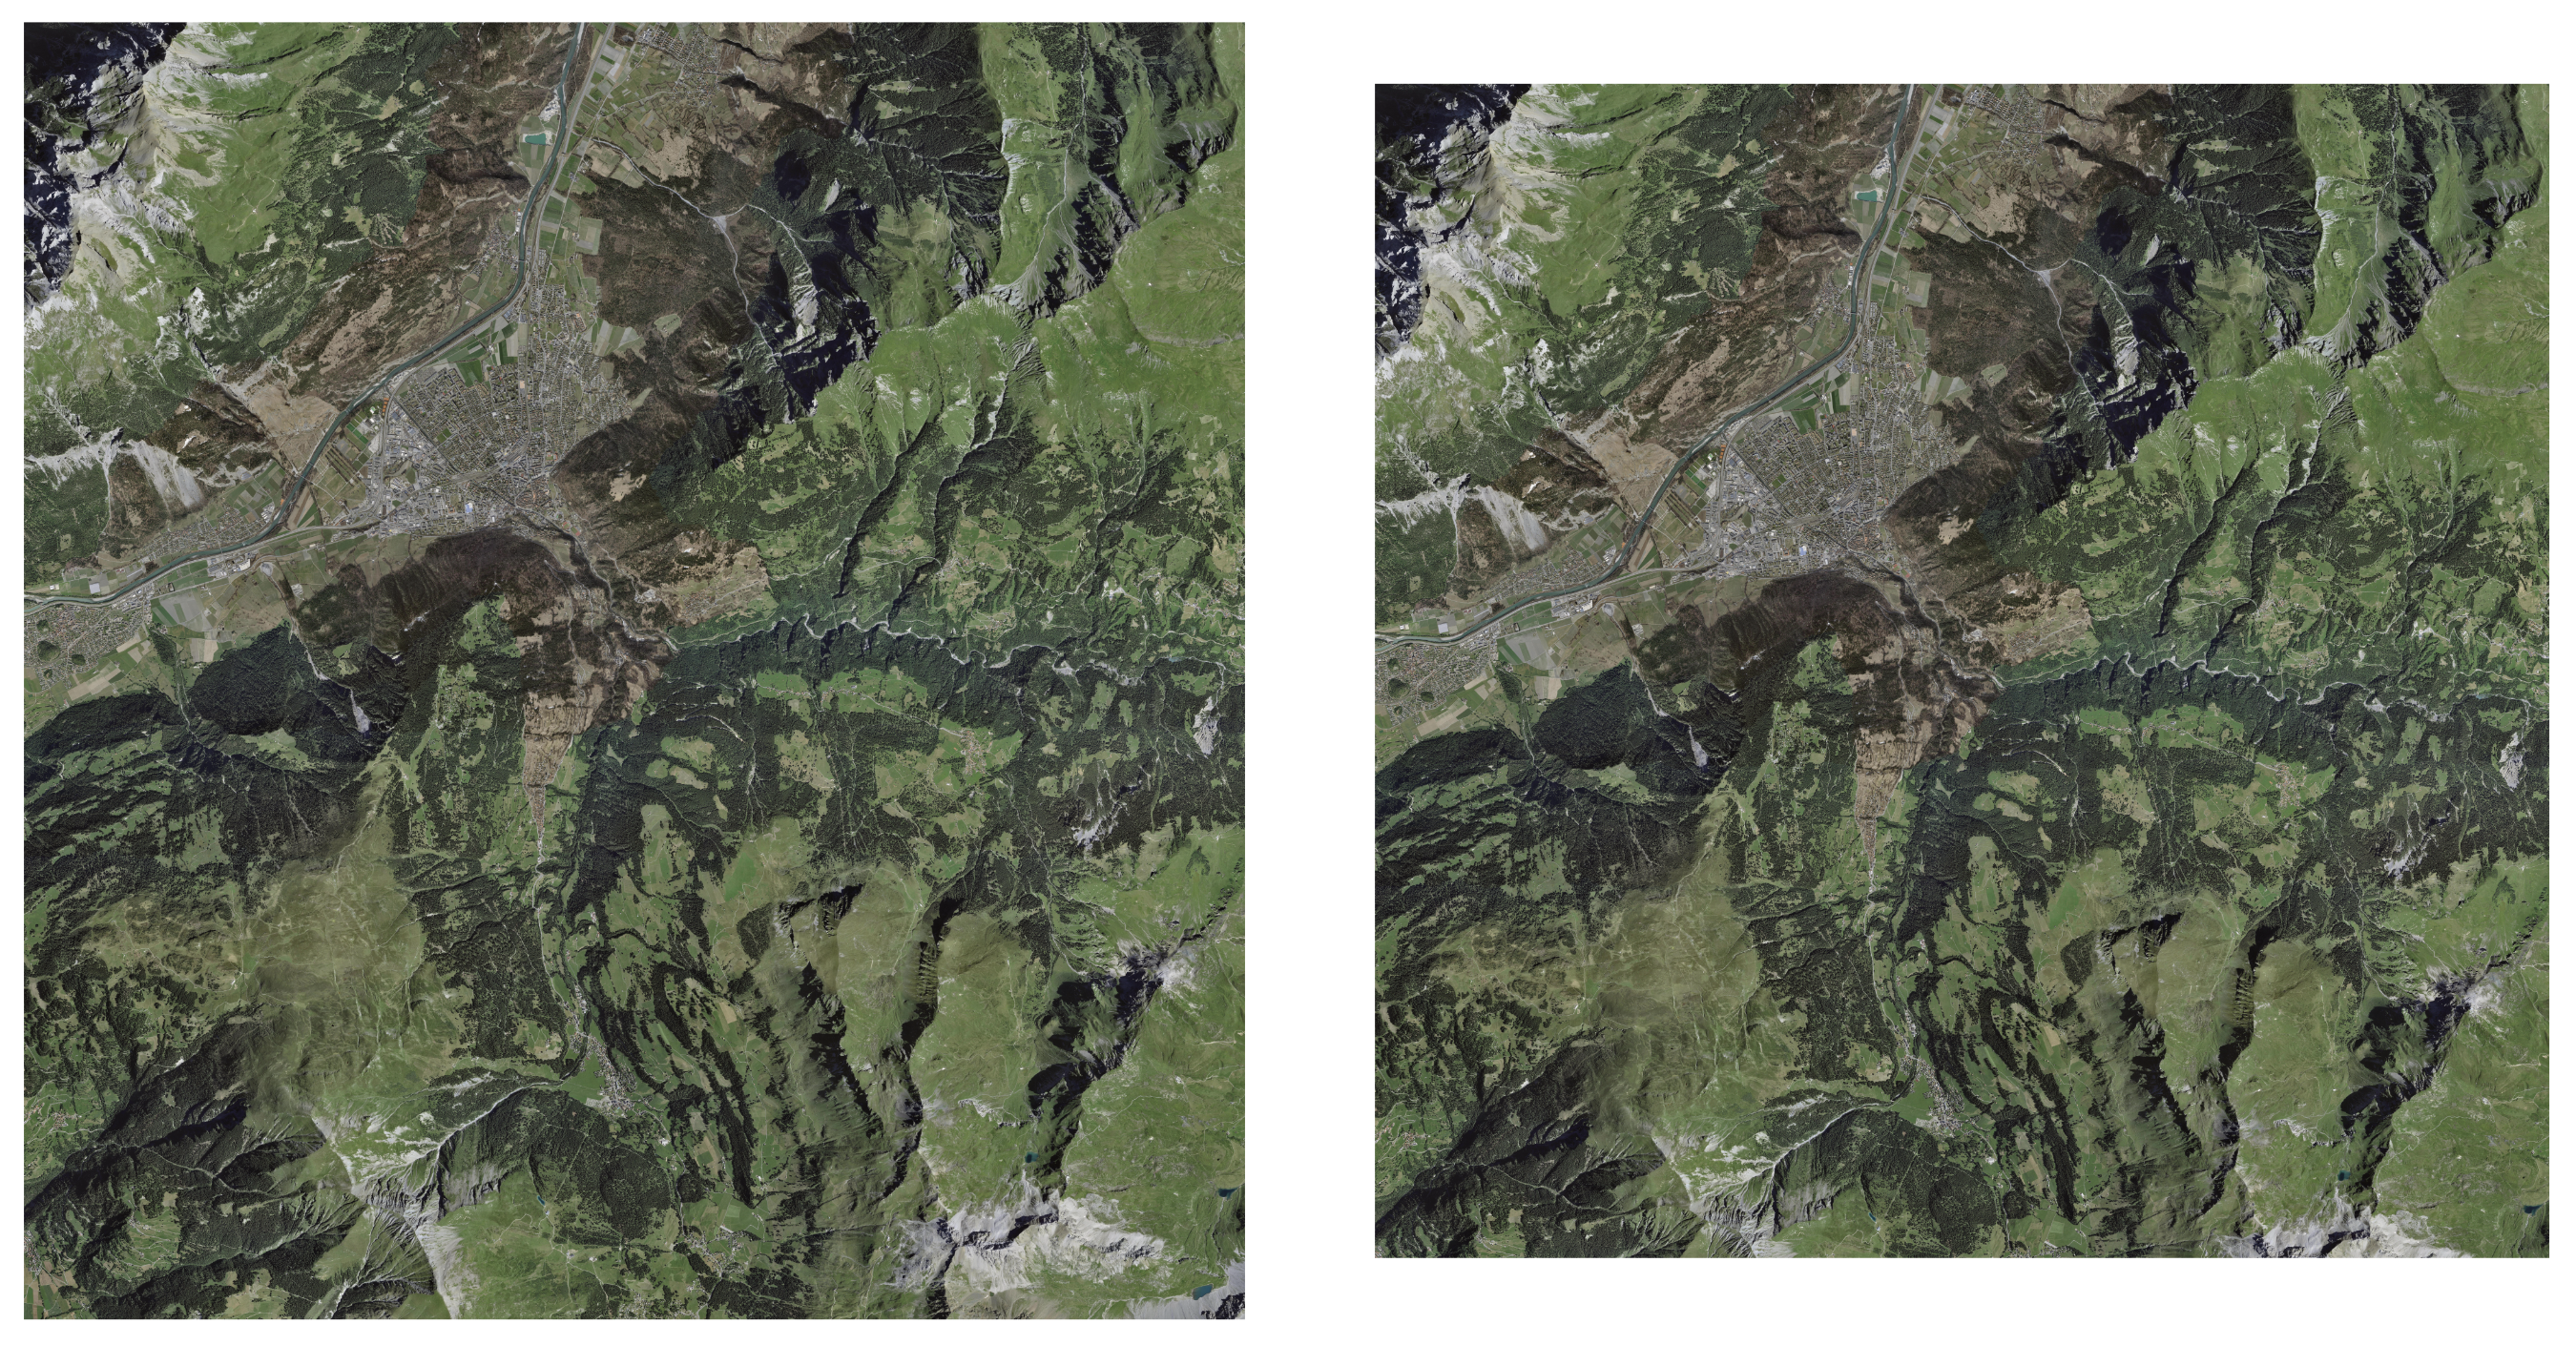
\includegraphics[width=.7\linewidth]{content/00_assets/begrenzung_bildausschnitt.png}
    \label{fig_begrenzung_bildausschnitt}
\end{figure}
Der quadratische Ausschnitt wird so gewählt, dass das Gesamtbild restlos durch Tiles in der höchsten Auflösung (LOD 2 in Abbildung \ref{fig_textur_teilbilder_quadtree}) aufgeteilt werden kann.

\subsection{Automatische Ermittlung der maximalen Baumtiefe}
\label{chap_ermittlung_baumtiefe}
Da die Tiles inspiriert vom Quadtree Algorithmus generiert werden, können die maximale Baumtiefe und somit die höchste Detailstufe im Vorfeld ermittelt werden. Hierzu ein Beispiel. Angenommen, das Luftbild von Sargans hat eine Auflösung ($R$) von 2000px auf 2000px. Des Weiteren gehen wir davon aus, dass die swisstopo Daten eine Auflösung von 2m pro Bildpunkt besitzen. Hierdurch ergibt sich eine Tile-Auflösung ($T$) von 500px ($\frac{1000m}{\frac{2m}{1px}}$) pro km$^2$. Die maximale Baumtiefe ($L_{\max}$) kann mithilfe der Logarithmusfunktion bestimmt werden. Anhand der beschriebenen Parameter würde sich daher für den Raum Sargans eine maximale Baumtiefe von 3 ergeben.
\[
L_{\max} = (\log_2\frac{R}{T}) + 1
\]

\subsection{Border Patching}
Mithilfe der extrahierten Höhen- und Bildinformationen ist es möglich, 3D-Modelle zu rekonstruieren. Auf die genaue Generierung der 3D-Modelle wird in Kapitel \ref{chap_erstellung_geometrie} eingegangen. Werden die Modelle aneinandergereiht, so wird ersichtlich, dass sich Risse an den Kanten bilden (siehe schwarze Bereiche in Abbildung \ref{fig_risse_zwischen_3d_modellen}). Diese Risse entstehen, weil die Höhenwerte an den Schnittkanten nicht mit den Höhenwerten der angrenzenden Nachbarn übereinstimmen. Dadurch divergieren die Position der Vertices und es bilden sich Risse.
\begin{figure}[H]
    \caption{Risse zwischen 3D Modellen der gleichen Detailstufe (Eigene Darstellung)}
    \includegraphics[width=.3\linewidth]{content/00_assets/risse_zwischen_gleichen_detailstufen.png}
    \label{fig_risse_zwischen_3d_modellen}
\end{figure}

Diese Problematik kann mithilfe des sogenannten ``Border Patching'' eliminiert werden. Hierzu werden jeweils an den Schnittkanten die Daten der angrenzenden Nachbarn übernommen und so ein Überlappungsbereich geschaffen. Bereits ein Bereich von einem Pixel reicht aus, um die Risse zu eliminieren. Abbildung \ref{fig_border_patching} stellt den Überlappungsbereich in Form von roten Linien dar. An diesen Kanten werden jeweils die Werte der Nachbarn (d.h. von 1 nach 2 etc.) übernommen.
\begin{figure}[H]
    \caption{Border Patching (Eigene Darstellung)}
    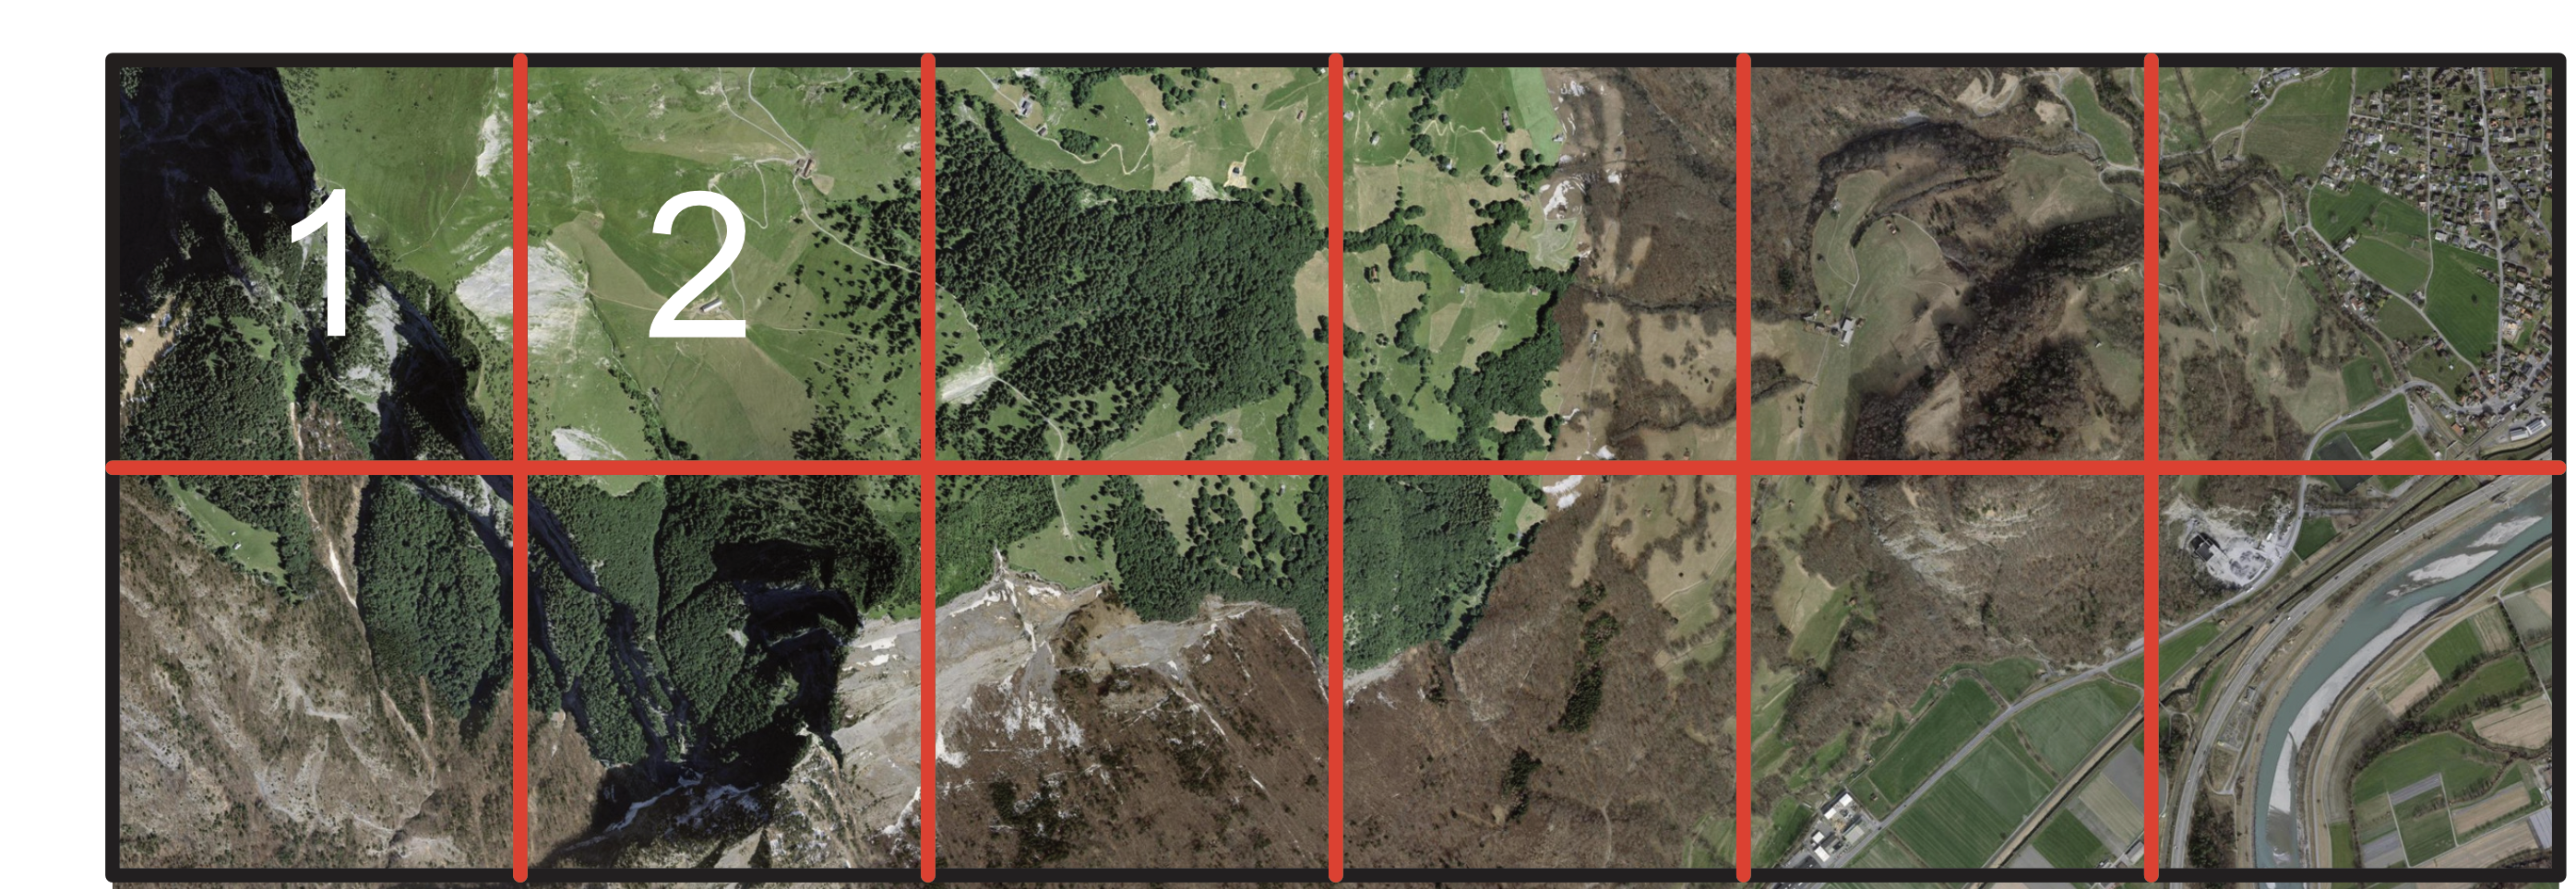
\includegraphics[width=.5\linewidth]{content/00_assets/border_patching.png}
    \label{fig_border_patching}
\end{figure}

\subsection{Relative Geopositionsinformationen}
Das Three.js Koordinatensystem weist einen anderen Koordinatenmittelpunkt (0/0) auf als die swisstopo Daten (2'600'000/1'200'000). Um die 3D-Modelle korrekt in Three.js zu positionieren, werden daher relative Geopositionsinformationen berechnet. Hierzu wird zuerst der Mittelpunkt des Gesamtbildes im LV95 Koordinatensystem bestimmt. Anschliessend wird für jede Tile der relative Abstand zu diesem Mittelpunkt ermittelt und in den Metadaten abgespeichert. Hiermit ist sichergestellt, dass die 3D-Modelle relativ um den Three.js Koordinatenmittelpunkt platziert werden können.

\subsection{Generierung von Metadaten}
\label{chap_generierung_metadaten}
Um wichtige Informationen in Bezug auf die swisstopo Daten nicht zu verlieren, werden entsprechende Metadaten generiert. Die Metadaten werden als JSON-Datei (siehe Abbildung \ref{fig_ausschnitt_metadaten}) abgespeichert und entsprechend zur Laufzeit der Webanwendung eingelesen. Tabelle \ref{table_metadata} gibt einen Überblick über die Metadaten sowie den Verwendungszweck.
\begin{table}[H]
    \caption{Erstellte Metadaten und Verwendungszweck (Eigene Darstellung)}
    \begin{tabularx}{\textwidth} {
        >{\raggedright\arraybackslash}X 
        >{\raggedright\arraybackslash}X}
            \hline
            \textbf{Metadaten} & {Verwendungszweck}  \\
            \hline
            Absolute Geopositionsinformationen (LV95) & LV95 Koordinaten der Tiles \\
            Relative Geopositionsinformationen (LV95) & Relative Positionierung der Tiles zum Three.js Koordinatenmittelpunkt \\
            Maximale Baumtiefe & Limitierungskriterium für den Quadtree Algorithmus \\
            Dateipfade zu den erstellten Bilddateien & Werden zur Laufzeit geladen und bilden die Grundlage für die 3D-Geometrien \\
            \hline
    \end{tabularx}
    \bigbreak
    \label{table_metadata}
\end{table}

\begin{figure}[H]
    \caption{Auszug aus den generierten Metadaten (Eigene Darstellung)}
    \includegraphics[width=.5\linewidth]{content/00_assets/ausschnitt_metadaten.png}
    \label{fig_ausschnitt_metadaten}
\end{figure}

\section{Implementierung}
Dieses Kapitel widmet sich der eigentlichen Implementierung der 3D-Terrainvisualisierung auf Basis des Three.js Frameworks und der swisstopo-Daten. Zu Beginn wird auf die Erstellung der eigentlichen 3D-Modelle anhand der vorverarbeiteten Daten eingegangen. Anschliessend werden die eingesetzten Algorithmen sowie entsprechende Hilfsvisualisierungen thematisiert. Abgerundet wird dieses Kapitel mit der Implementierung der Steuerungselemente zur freien Bewegung im 3D-Raum. Die Terrainvisualisierung steht unter der MIT-Lizenz und ist auf GitHub\footnote{\url{https://github.com/yhutter/swiss-terrain-3d}} verfügbar.

\subsection{Erstellung der 3D-Geometrie}
\label{chap_erstellung_geometrie}
Um das Gebirge in 3D zu visualisieren, wird für die Geometrie ein Gitternetz von Punkten eingesetzt. In Three.js wird hierzu die sogenannte ``PlaneGeometry'', welche eine Ebene im 3D-Raum darstellt, verwendet (siehe Abbildung \ref{fig_threejs_plane_geometry}). Die Auflösung dieser Geometrie kann beliebig verfeinert werden, wodurch schlussendlich ein Gitternetz entsteht.
\begin{figure}[H]
    \caption{Three.js PlaneGeometry \parencite{threejs_beispiel_plane_geometry_2025}}
    \includegraphics[width=.3\linewidth]{content/00_assets/threejs_plane_geometry.png}
    \label{fig_threejs_plane_geometry}
\end{figure}

Um Risse im Terrain zwischen verschiedenen LOD's zu vermeiden, wird anstelle eines diagonalen ein sternförmiges Muster (siehe Abbildung \ref{fig_plane_geometry_star_structure}) verwendet. In Kombination mit dem sogenannten ``Index-Stitching'' lassen sich hierdurch Risse eliminieren (die genaue Erläuterung folgt in Kapitel \ref{chap_quadtree_algorithmus}). 
\begin{figure}[H]
    \caption{Gitternetz mit sternförmiger Struktur \parencite[S. 54]{frostbite_terrain_rendering_2007}}
    \includegraphics[width=.3\linewidth]{content/00_assets/geometry_star_pattern.png}
    \label{fig_plane_geometry_star_structure}
\end{figure}

Obwohl Three.js viele 3D-Geometrien zur Verfügung stellt, ist es ebenso möglich, eigene Geometrien zu definieren. Hierfür stellt Three.js die Klasse \textit{BufferGeometry} zur Verfügung. Um die gewünschte sternförmige Struktur zu konstruieren, wurde hiermit eine eigene Geometrie definiert. Wie in Kapitel \ref{chap_render_pipelines} erwähnt, bestehen 3D-Modelle aus Dreiecken, welche wiederum aus Punkten (Vertices) bestehen. Um die Reihenfolge festzulegen, wie die einzelnen Punkte zu Dreiecken zusammengesetzt werden, stehen sogenannte ``Indices'' zur Verfügung. Hierzu ein Beispiel mit Bezug auf Abbildung \ref{fig_create_geometry_with_indices}. Um das Dreieck $abi$ zu erstellen, muss zuerst der Punkt $a$ mit dem Punkt $b$ und schlussendlich mit dem Punkt $i$ verbunden werden. Dies wird für sämtliche Dreiecke wiederholt, bis die gewünschte sternförmige Struktur entsteht. 
\begin{figure}[H]
    \caption{Erstellung der Geometrie mittels Indices (Eigene Darstellung)}
    \includegraphics[width=.7\linewidth]{content/00_assets/erstellung_geometry_mittels_indices.png}
    \label{fig_create_geometry_with_indices}
\end{figure}

Momentan befinden sich jedoch noch alle Punkte auf einer Ebene. Um ein 3D-Modell zu erhalten, müssen die Punkte anhand der extrahierten Höhendaten entsprechend nach oben oder unten verschoben werden. Die Verschiebung der Punkte erfolgt im Vertex Shader (siehe Kapitel \ref{chap_render_pipelines}). Hierbei werden die Höhenwerte aus den Graustufenbildern gelesen und anhand des vorberechneten globalen Maximum- und Minimumhöhenwerts entsprechend skaliert. Die Vertices der Geometrie werden anschliessend anhand dieses Wertes entsprechend verschoben (siehe Abbildung \ref{fig_verschiebung_punkte_vertex_shader}). Der Code in Abbildung \ref{fig_verschiebung_punkte_vertex_shader} ist in einer Three.js spezifischen Programmiersprache für Shader mit dem Namen \acrfull{TSL} geschrieben. Wie in Kapitel \ref{chap_technologien} thematisiert, unterstützt Three.js sowohl WebGL als auch die neuere WebGPU Grafikschnittstelle. Die Programmiersprache dieser zwei Schnittstellen ist jedoch unterschiedlich. \acrshort{TSL} fungiert hier als ``Übersetzer'' zwischen diesen Sprachen und erlaubt es somit, beide Grafikschnittstellen mit derselben Programmiersprache anzusprechen. Hierbei wird von Three.js je nach Hardwaresupport die geeignetste Grafikschnittstelle ausgewählt. 
\begin{figure}[H]
    \caption{Verschiebung der Punkte im Vertex Shader (Eigene Darstellung)}
    \includegraphics[width=.9\linewidth]{content/00_assets/positionierung_punkte_vertex_shader.png}
    \label{fig_verschiebung_punkte_vertex_shader}
\end{figure}

\subsection{Texturierung der 3D-Geometrie}
\label{chap_texturierung_3d_geometrie}
Um 3D-Modelle in Three.js darzustellen, wird nebst der eigentlichen Geometrie auch ein sogenanntes ``Material'' benötigt. Die Geometrie alleine gibt dem 3D-Modell die notwendige Struktur, das Material, welches über die Geometrie gelegt wird, das finale Erscheinungsbild. Für ein Material können nebst einer Textur auch diverse andere Dinge verschiedene Farben verwendet werden. Um in Three.js etwa einen Würfel in grüner Farbe darzustellen, werden eine \textit{BoxGeometry} sowie ein \textit{MeshBasicMaterial} mit der entsprechenden Farbe benötigt (siehe Abbildung \ref{fig_threejs_box}).
\begin{figure}[H]
    \caption{Beispielcode zur Erstellung eines Würfels in Three.js \parencite{threejs_beispiel_box_geometry_2025}}
    \includegraphics[width=.9\linewidth]{content/00_assets/threejs_beispiel_box.png}
    \label{fig_threejs_box}
\end{figure}

Analog zum vorherigen Beispiel kann auch die 3D-Geometrie eines Gebirges mit einer Textur versehen werden. Die Texturen sind in diesem Fall die orthografisch korrigierten Luftbilder aus dem swissIMAGE-Datensatz. Hierzu werden im Fragment Shader (siehe Kapitel \ref{chap_render_pipelines}) die entsprechenden Pixelwerte der Luftbilder ausgelesen und als Farbe dargestellt. Das Endergebnis ist ein rekonstruiertes 3D-Modell auf Basis einer Kombination von swissALTI3D (Höhenwerte) sowie swissIMAGE (Texturen) Daten. 
\begin{figure}[H]
    \caption{Ausschnitt rekonstruiertes 3D-Modell auf Basis der swisstopo-Daten (Eigene Darstellung)}
    \includegraphics[width=.5\linewidth]{content/00_assets/texturiertes_3d_modell.png}
    \label{fig_texturiertes_3d_modell}
\end{figure}

\subsection{Quadtree Algorithmus}
\label{chap_quadtree_algorithmus}
Als Hauptalgorithmus hat sich der Autor für einen Quadtree entschieden. Hauptgrund hierfür war die einfachere Implementierung im Vergleich zum Geometry Clipmap sowie CDLOD Algorithmus. Wie in Kapitel \ref{chap_algorithmen} angesprochen, benötigt ein Quadtree ein Kriterium, welches festlegt, wann neue Nodes generiert werden. Hierfür wird die euklidische Distanz von der Kameraposition zum Mittelpunkt einer Node verwendet (siehe Abbildung \ref{fig_quadtree_split_metric}). Zusätzlich wird der Quadtree anhand der vorberechneten Baumtiefe (siehe Kapitel \ref{chap_ermittlung_baumtiefe}) entsprechend limitiert. Als Input für den Quadtree werden die Länge sowie die Breite des Gebirges verwendet. Zur Laufzeit wird jeweils die Kameraposition in den Quadtree eingefügt und entsprechend die Abstände zu den einzelnen Nodes berechnet.
\begin{figure}[H]
    \caption{Quadtree Kriterium zur Erstellung neuer Nodes (Eigene Darstellung)}
    \includegraphics[width=.8\linewidth]{content/00_assets/quadtree_split_metric.png}
    \label{fig_quadtree_split_metric}
\end{figure}

\subsubsection{Assoziierung zu den Metadaten}
Die einzelnen Nodes des Quadtrees enthalten Informationen über das räumliche Gebiet sowie die dazugehörige Baumtiefe. Damit aus den einzelnen Nodes die dazugeöhrigen 3D Modelle rekonstruiert werden können, müssen diese Informationen mit den erstellten Metadaten (siehe Kapitel \ref{chap_generierung_metadaten}) verknüpft werden. Die Verknüpfung erfolgt anhand des Node-Mittelpunktes (Zentrum des räumlichen Gebietes) sowie der dazugehörigen Baumtiefe (siehe Abbildung \ref{fig_assoziierung_quadtree_node_metadaten}). 
\begin{figure}[H]
    \caption{Assoziierung Quadtree Node zu den Metadaten (Eigene Darstellung)}
    \includegraphics[width=.7\linewidth]{content/00_assets/assoziierung_quadtreenode_metadaten.png}
    \label{fig_assoziierung_quadtree_node_metadaten}
\end{figure}

Der Node-Mittelpunkt wird anhand des Feldes \textit{bbox\_world\_space} berechnet, wobei die Baumtiefe dem Feld \textit{level} entspricht (siehe Abbildung \ref{fig_ausschnitt_metadaten_tile}). Aufgrund dieser Kriterien wird in den Metadaten nach einem entsprechenden Eintrag gesucht und schlussendlich ein 3D-Modell erstellt. Da sich die Struktur des Quadtrees abhängig von der Kameraposition ändert, wird ebenfalls sichergestellt, dass nicht mehr verwendete Modelle entfernt werden.
\begin{figure}[H]
    \caption{Ausschnitt Tile Metadaten (Eigene Darstellung)}
    \includegraphics[width=.7\linewidth]{content/00_assets/ausschnitt_metadaten_tile.png}
    \label{fig_ausschnitt_metadaten_tile}
\end{figure}

\subsubsection{Risse zwischen Nodes mit unterschiedlicher Baumtiefe}
\label{chap_visuelle_diskrepanz_zwischen_nodes}
Je nach Baumtiefe erstrecken sich die einzelnen Nodes über einen grösseren Bereich. Für jede Node wird die gleiche Geometrie verwendet (siehe Kapitel \ref{chap_erstellung_geometrie}). Treffen Geometrien mit einer unterschiedlichen Baumtiefe aufeinander, entstehen visuelle Diskrepanzen in Form von Rissen (siehe rote Bereiche in Abbildung \ref{fig_visuelle_diskrepanzen_zwischen_unterschiedlichen_lod_leveln}). 
\begin{figure}[H]
    \caption{Visuelle Diskrepanzen zwischen Geometrien mit einer unterschiedlichen Baumtiefe \parencite{frostbite_terrain_rendering_2007}}
    \includegraphics[width=.4\linewidth]{content/00_assets/lod_tjunctions.png}
    \label{fig_visuelle_diskrepanzen_zwischen_unterschiedlichen_lod_leveln}
\end{figure}

Die Risse entstehen, weil kleinere Geometrien zusätzliche Vertices aufweisen, welche nicht auf jene der grösseren Geometrien passen. Diese zusätzlichen Vertices werden im Vertex Shader ebenfalls nach unten oder oben verschoben, wodurch sich Risse bilden (siehe Abbildung \ref{fig_risse_zwischen_3d_modellen_unterschiedlicher_baumtiefe}).
\begin{figure}[H]
    \caption{Risse zwischen 3D-Modellen unterschiedlicher Baumtiefe (Eigene Darstellung)}
    \includegraphics[width=.5\linewidth]{content/00_assets/risse_zwischen_unterschiedlichen_baumtiefen.png}
    \label{fig_risse_zwischen_3d_modellen_unterschiedlicher_baumtiefe}
\end{figure}

\newpage
Um diese Problematik zu lösen, wird das sogenannte ``Index-Stitching'' der Frostbite Engine verwendet. Wie in Kapitel \ref{chap_erstellung_geometrie} erwähnt, erlauben \textit{Indices} festzulegen, wie die einzelnen Vertices zu Dreiecken zusammengesetzt werden. Mithilfe dieser Indices können jedoch auch einzelne Punkte übersprungen werden. Auf diesem Ansatz basiert das Index-Stitching. Hierzu werden im Vorfeld neun unterschiedliche Index-Buffer, welche die einzelnen Indices beinhalten, berechnet (siehe Abbildung \ref{fig_frostbite_index_stitching}). Zur Laufzeit der Anwendung wird jeweils überprüft, welcher der neun Index-Buffer auf die einzelnen Geometrien angewendet werden muss, um die Risse zu eliminieren.
\begin{figure}[H]
    \caption{Frostbite Engine Index-Stitching \parencite[S. 55]{frostbite_terrain_rendering_2007}}
    \includegraphics[width=.5\linewidth]{content/00_assets/frostbite_index_stitching.png}
    \label{fig_frostbite_index_stitching}
\end{figure}

Um den korrekten Index-Buffer zu bestimmen, werden für jede Node im Quadtree die angrenzenden Nachbarn ermittelt. Nachbarn derselben Baumtiefe werden ignoriert. Je nachdem, auf welcher Kante die Nachbarn liegen, wird anschliessend der entsprechende Index-Buffer ausgewählt (siehe Abbildung \ref{fig_auswahl_index_stitching}).
\begin{figure}[H]
    \caption{Ermittlung Index-Stitching (Eigene Darstellung)}
    \includegraphics[width=.5\linewidth]{content/00_assets/ermittlung_index_stitching_mode.png}
    \label{fig_auswahl_index_stitching}
\end{figure}

Abbildung \ref{fig_wireframe_index_stitching} zeigt eine Wireframe-Ansicht zweier angrenzender Geometrien mit einer unterschiedlichen Baumtiefe. Wie an den Rändern zu erkennen ist, gibt es keine zusätzlichen Vertices mehr und die Geometrien passen korrekt aneinander.
\begin{figure}[H]
    \caption{Wireframe-Ansicht für Index-Stitching (Eigene Darstellung)}
    \includegraphics[width=.4\linewidth]{content/00_assets/index_stitching_wireframe.png}
    \label{fig_wireframe_index_stitching}
\end{figure}

Eine Limitation des Index-Stitching besteht darin, dass sichergestellt werden muss, dass sich die Baumtiefe angrenzender Quadtree Nodes nur um eine Stufe unterscheiden darf \parencite[S. 53]{frostbite_terrain_rendering_2007}. Hierfür wird der Quadtree entsprechend ausbalanciert.

\subsubsection{Hilfsvisualisierung}
Um sowohl die Korrektheit des Quadtrees als auch der Index-Stitching Methode zu überprüfen, wurde eine Hilfsvisualisierung implementiert. Die einzelnen Nodes des Quadtrees werden als weisse Linien dargestellt. Nodes, bei denen ein Index-Stitching notwendig ist, sind durch rote Linien gekennzeichnet (siehe Abbildung \ref{fig_hilfsvisualisierung_quadtree_index_stitching}).
\begin{figure}[H]
    \caption{Hilfsvisualisierung für Quadtree und Index-Stitching Überprüfung (Eigene Darstellung)}
    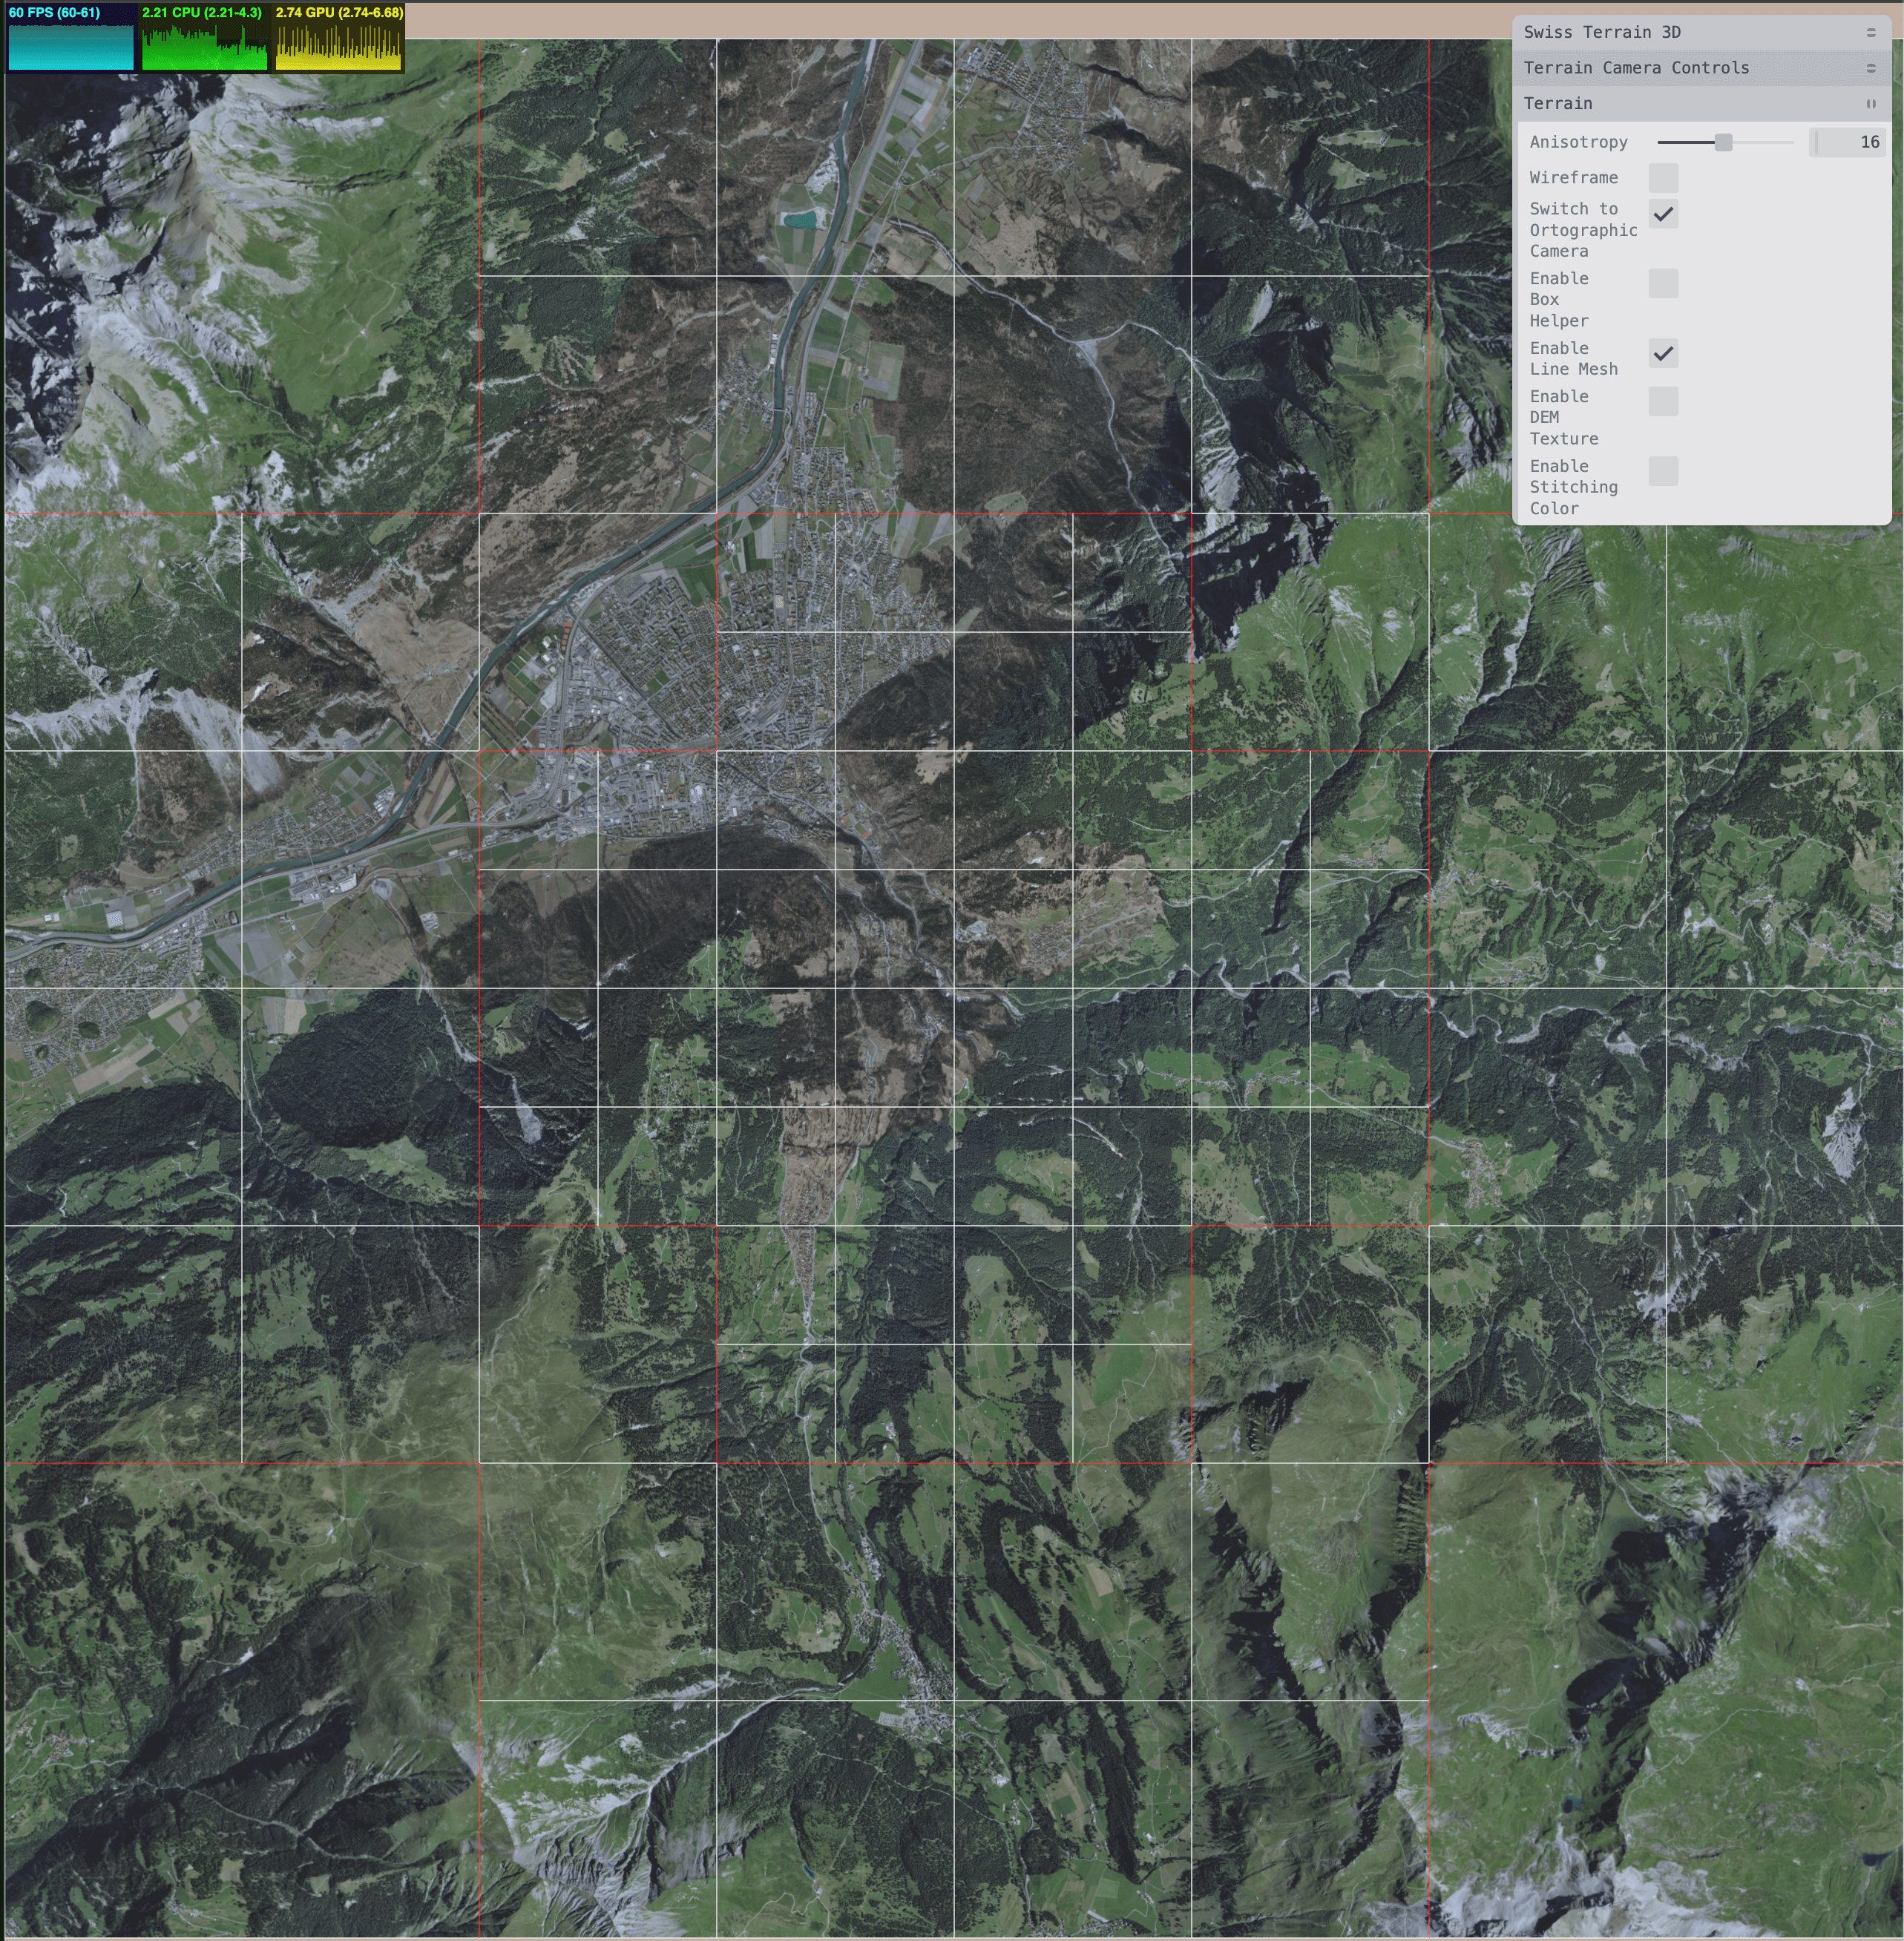
\includegraphics[width=.4\linewidth]{content/00_assets/hilfsvisualisierung_quadtree.png}
    \label{fig_hilfsvisualisierung_quadtree_index_stitching}
\end{figure}

\subsection{Steuerungselemente}
\label{chap_steuerungselemente}
Damit eine freie Bewegung durch das Gebirge möglich ist, müssen entsprechende Steuerungselemente implementiert werden. Der Betrachtungsausschnitt der Visualisierung wird hierbei durch eine Kamera definiert. In Three.js stehen verschiedene Arten von Kameras zur Verfügung. Eine ``Perspective Camera'' wird beispielsweise eingesetzt, um Objekte im 3D-Raum darzustellen. Hierbei erscheinen die entsprechenden Objekte, abhängig von der Distanz zur Kamera, entsprechend grösser oder kleiner. Die ``Ortographic Camera'' stellt alle Objekte unabhängig von der Distanz gleich gross dar (siehe Abbildung \ref{fig_threejs_cameras}). Aus diesen Gründen wird für die Terrainvisualisierung eine Perspective Camera und für Hilfsvisualisierung eine Ortographic Camera verwendet. 
\begin{figure}[H]
    \caption{Verschiedene Arten von Kameras in Three.js \parencite{threejs_exploring_cameras_2023}}
    \includegraphics[width=.5\linewidth]{content/00_assets/threejs_cameras.png}
    \label{fig_threejs_cameras}
\end{figure}

Mithilfe von Maus und Tastatur können sowohl die Position als auch der Betrachtungswinkel der Kameras verändert werden und erlauben hiermit eine freie Bewegung durch die Terrainvisualisierung. Tabelle \ref{table_steuerungselemente} zeigt eine Übersicht der Steuerungselemente und deren Auswirkung.
\begin{table}[H]
    \caption{Übersicht über Steuerungselemente und deren Auswirkung (Eigene Darstellung)}
    \begin{tabularx}{\textwidth} {
        >{\raggedright\arraybackslash}X 
        >{\raggedright\arraybackslash}X}
            \hline
            \textbf{Steuerungselement} & {Auswirkung}  \\
            \hline
            W-Taste oder Pfeiltaste nach oben & Bewegung nach vorne \\
            A-Taste oder Pfeiltaste nach link & Bewegung nach links \\
            S-Taste oder Pfeiltaste nach unten & Bewegung nach hinten \\
            D-Taste oder Pfeiltaste nach rechts & Bewegung nach rechts \\
            E-Taste & Bewegung nach oben \\
            R-Taste & Bewegung nach unten \\
            Mausbewegung & Veränderung des Betrachtungswinkels \\
            \hline
    \end{tabularx}
    \bigbreak
    \label{table_steuerungselemente}
\end{table}

\section{Ästhetik}
Three.js bietet diverse Möglichkeiten, um die Ästhetik einer 3D-Visualisierung zu beeinflussen. Ziel dieses Kapitels ist es, einen Überblick über die verwendeten ästhetischen Anpassungen, sowie deren Einfluss, zu geben.

\subsection{\acrfull{HDR} und Tone Mapping}
\acrfull{HDR} im Kontext von Bildern erlaubt es das Helligkeitsspektrum der einzelnen Farben, feingranularer darzustellen. Standardmässig sind die Farben eines Bildes nur innerhalb eines bestimmten Spektrums unterscheidbar. Farben, welche sich in den hellsten Bereichen des Spektrums befinden, werden weiss dargestellt, wohingegen Farben im niedrigsten Spektrum schwarz dargestellt werden. Die Spanne dieses Spektrums wird als Dynamic Range bezeichnet. Dadurch, dass diese Spannweite bei \acrshort{HDR} erheblich grösser und feingranularer ist, werden die Helligkeitsunterschiede besser repräsentiert \parencite{hdr_2022}. Abbildung \ref{fig_terrain_hdr_no_hdr} zeigt die entsprechenden Kontrastunterschiede.

\begin{figure}[H]
    \caption{Kontrastunterschied der Gebirge mit HDR (links) und ohne (rechts) (Eigene Darstellung)}
    \includegraphics[width=1.0\linewidth]{content/00_assets/terrain_hdr_no_hdr.png}
    \label{fig_terrain_hdr_no_hdr}
\end{figure}

Um \acrshort{HDR} Bilder zu erstellen, gibt es mehrere Möglichkeiten. Zum einen können die Bilder mithilfe des Computers erstellt werden, zum anderen ist es auch möglich, ein \acrshort{HDR} Bild auf Basis von mehreren Einzelbildern mithilfe von speziellen Kamerasensoren zu erstellen \parencite{hdr_2022}. Darüber hinaus gibt es spezialisierte Webseiten wie Poly Haven\footnote{\url{https://polyhaven.com/hdris}} womit HDR Bilder direkt heruntergeladen werden können.

Damit die Farbwerte von HDR Bildern auf dem Bildschirm dargestellt werden können, müssen sie in ein darstellbares Spektrum überführt werden. Um dies zu bewerkstelligen, wird das sogenannte ``Tone Mapping'' verwendet. Three.js unterstützt hierbei Tone Mapping-Verfahren. Abbildung \ref{fig_tone_mapping_threejs} zeigt die Auswirkungen von verschiedenen Tone Mapping-Verfahren auf die finale Darstellung.

\begin{figure}[H]
    \caption{Verschiedene Tone Mapping-Verfahren in Three.js von links nach rechts (Kein Tone Mapping, Agx, Filmic, Reinhard) (Eigene Darstellung)}
    \includegraphics[width=.8\linewidth]{content/00_assets/tone_mapping_threejs.png}
    \label{fig_tone_mapping_threejs}
\end{figure}

\subsection{Anisotropy}
Um die Performance zu erhöhen, können für Texturen sogenannte ``Mipmaps'' erstellt werden. Mipmaps sind herunterskalierte Versionen der Originaltextur (siehe Abbildung \ref{fig_mipmaps}). Die Grafikkarte selektiert je nach Blickwinkel und Abstand die passende Mipmap Textur. Mit dieser Methode werden automatisch kleinere (herunterskalierte) Versionen für Dinge genutzt, welche sich in der Ferne befinden \parencite{mipmaps_2023}.
\begin{figure}[H]
    \caption{Mipmaps \parencite{mipmaps_2023}}
    \includegraphics[width=.3\linewidth]{content/00_assets/mipmaps.jpg}
    \label{fig_mipmaps}
\end{figure}

Jedoch kann es bei der Verwendung von Mipmaps dazu führen, dass Texturen, welche sich in der Ferne befinden, kaum mehr erkennbar sind oder unscharf erscheinen. Um dieses Problem zu lösen, gibt es die Möglichkeit, mithilfe der sogenannten ``Anisotropy'' zu definieren, wie oft die einzelnen Bildpunkte einer Mipmap gefiltert werden sollen \parencite{threejs_anisotropy_2025}. Hiermit können verwaschene und unscharfe Texturen vermieden werden (siehe rote Bereiche A und B in Abbildung \ref{fig_anisotropy}).
\begin{figure}[H]
    \caption{Texturen mit Anisotropy (links) und ohne (rechts) (Eigene Darstellung)}
    \includegraphics[width=1.0\linewidth]{content/00_assets/textur_mit_anisotropy_ohne.png}
    \label{fig_anisotropy}
\end{figure}

\subsection{Procedural Sky}
Das Three.js Ökosystem bietet eine Vielzahl von verschiedenen Modulen an, um realitätsnahe Visualisierungen zu ermöglichen. Mithilfe des \textit{Procedural Sky}\footnote{\url{https://threejs.org/examples/?q=sky#webgpu_sky}} Plugins kann beispielsweise ein Tag- und Nachtzyklus simuliert werden. Das Plugin bietet hierzu diverse Einstellungsmöglichkeiten, womit wichtige Elemente wie die Sonnenposition etc. eingestellt werden können. Dies ermöglicht es, das Gebirge in einer realitätsnahen Umgebung in Szene zu setzen. Abbildung \ref{fig_procedural_sky} zeigt den Einfluss des Procedural Sky Plugins auf das Gebirge. Das linke Bild stellt das Gebirge ohne Procedural Sky dar, wohingegen das mittlere und rechte Bild das Gebirge mit Procedural Sky aber jeweils mit unterschiedlichen Sonnenpositionen visualisieren.
\begin{figure}[H]
    \caption{Gebirge mit Procedural Sky Plugin (Eigene Darstellung)}
    \includegraphics[width=1.0\linewidth]{content/00_assets/threejs_procedural_sky.png}
    \label{fig_procedural_sky}
\end{figure}

\subsection{Einstellungsmöglichkeiten}
Die bis anhin besprochenen ästhetischen Elemente besitzen eine Vielzahl von verschiedenen Parametern. Um ein Gefühl dafür zu bekommen, welche Auswirkungen die Parameter haben und wie sich dadurch die visuelle Ästhetik verändert, ist es wichtig, dass diese in Echtzeit mithilfe von entsprechenden GUI-Elementen verändert werden können. Um Einstellungsparameter mit entsprechenden GUI-Elementen zu verknüpfen, stehen diverse Bibliotheken zur Verfügung. Eine populäre Bibliothek in der Three.js-Community ist Tweakpane\footnote{\url{https://tweakpane.github.io/docs/}}. Tweakpane bietet eine Vielzahl von unterschiedlichen GUI-Elementen wie Range-Slider, Color-Picker oder Accordions an. Tweakpane stellt zudem eine einheitliche Darstellung dieser Elemente zwischen den einzelnen Browsern sicher und ermöglicht es ebenfalls, die Elemente mithilfe von Themes\footnote{\url{https://tweakpane.github.io/docs/theming/}} entsprechend anzupassen. Der primäre Vorteil von Tweakpane gegenüber den standardmässigen HTML5-GUI-Elementen besteht darin, dass auf einfache Art und Weise eine Verknüpfung von Einstellungsparametern mit den GUI-Elementen möglich ist. Um ein Dropdown für die Auswahl des Tone-Mappings zu erstellen, müssen lediglich die Auswahloptionen sowie die Aktion, welche ausgeführt werden soll, wenn ein Element selektiert wird, definiert werden (siehe Abbildung \ref{fig_tweaks_code}).
\begin{figure}[H]
    \caption{Definitionsstruktur für ein Dropdown in Tweakpane (Eigene Darstellung)}
    \includegraphics[width=.6\linewidth]{content/00_assets/tweaks_beispiel_code.png}
    \label{fig_tweaks_code}
\end{figure}

Durch diese einfache Handhabung können schnell neue Elemente für wichtige Parameter definiert werden. Abbildung \ref{fig_tweaks} zeigt diverse GUI-Elemente (Tweaks), mithilfe derer diverse Aspekte der Terrain-Visualisierung in Echtzeit angepasst werden können.
\begin{figure}[H]
    \caption{Tweaks der Terrain-Visualisierung (Eigene Darstellung)}
    \includegraphics[width=.3\linewidth]{content/00_assets/tweaks.png}
    \label{fig_tweaks}
\end{figure}

\section{Performanz}
Im Rahmen dieses Kapitels wird die Performanz der Visualisierung evaluiert. Ausgehend davon werden entsprechende Engpässe aufgedeckt und hierfür durchgeführte Optimierungen besprochen. Die Messung erfolgte auf einem Macbook Pro M3 Max mit 64GB Arbeitsspeicher. Als Gebirge wurde der Raum Chur über ein Gebiet von 16 km$^2$ verwendet. 

\subsection{Im Vorfeld vorgenommene Optimierungen}
Vor der eigentlichen Messung, sind bereits einige Optimierungen im Vorfeld vorgenommen worden. Nachfolgend wird kurz auf die wichtigsten Optimierungen eingegangen.

\subsubsection{Webworker für Quadtree-Algorithmus}
Der Browser erlaubt standardmässig nicht das Ausführen von JavaScript-Code in mehreren Threads. Dies bedeutet, dass kostspielige Operationen die Visualisierung blockieren und so Verzögerungen auftreten können. Mithilfe von sogenannten ``Webworker'' ist es jedoch möglich, kostspielige Operationen in einem anderen Thread und somit im Hintergrund auszuführen. Dies ist jedoch mit gewissen Limitationen verbunden. Der Code hat beispielsweise keinerlei Zugriff auf das \acrfull{DOM} des Browsers. Dies untersagt unter anderem das Laden von Texturen. Jedoch können Algorithmen wie der Quadtree in Webworker ausgelagert werden. Hierdurch können sowohl die Berechnung des Quadtree als auch das notwendige Ausbalancieren im Hintergrund laufen, während der Main-Thread sich auf das Aktualisieren und Darstellen der hierauf aufbauenden 3D-Modelle fokussieren kann.

\subsubsection{Vorladen der Texturen}
Damit die Texturen der einzelnen Quadtree Nodes nicht dynamisch nachgeladen werden müssen, werden diese bereits zum Start der Applikation entsprechend vorgeladen. Obwohl dies zu Beginn für eine längere Wartezeit sorgt, hat dies zur Laufzeit den Vorteil, dass die Bilder sofort verfügbar sind und es somit nicht zu Ladeverzögerungen kommt.

\subsubsection{Frustum Culling}
Wie in Kapitel \ref{chap_steuerungselemente} erwähnt, unterstützt Three.js verschiedene Arten von Kameras. Diese Kameras haben ein definiertes Sichtfeld (Frustum). Um Rechenleistung zu sparen, werden Dinge, welche sich ausserhalb dieses Sichtfeldes befinden, nicht gezeichnet. Dies wird auch als ``Frustum Culling'' bezeichnet. Damit detektiert werden kann, ob sich ein Objekt innerhalb oder ausserhalb des Sichtfeldes befindet, nutzt Three.js sogenannte ``Bounding Spheres''. Diese muss zur Laufzeit für jede Geometrie entsprechend berechnet werden. Als Grundlage für die Berechnung der Bounding Sphere wird eine ``Bounding Box'' verwendet. Eine Bounding Box ist ein dreidimensionaler Bereich, welcher die 3D-Geometrie umschliesst (siehe rote Bereiche in Abbildung \ref{fig_bounding_boxes}).
\begin{figure}[H]
    \caption{Visualisierung der Bounding Box (Eigene Darstellung)}
    \includegraphics[width=.4\linewidth]{content/00_assets/terrain_bounding_boxes.png}
    \label{fig_bounding_boxes}
\end{figure}
Die Bounding Box wird aufgrund der globalen Höhenwerte des Gebirges sowie der räumlichen Abdeckung der Quadtree Nodes berechnet. Auf Basis dieses Bereiches kann anschliessend die für das Frustum Culling notwendige Bounding Sphere berechnet werden (siehe Abbildung \ref{fig_berechnung_bounding_box}).

\begin{figure}[H]
    \caption{Berechnung der Bounding Box (Eigene Darstellung)}
    \includegraphics[width=.5\linewidth]{content/00_assets/berechnung_bbox.png}
    \label{fig_berechnung_bounding_box}
\end{figure}

\subsubsection{Vorberechnung der Geometrie}
Die grundlegende Geometrie der einzelnen Quadtree Nodes ist identisch. Die Geometrien unterscheiden sich nur in der Grösse sowie im Index-Stitching Verfahren (siehe Kapitel \ref{chap_visuelle_diskrepanz_zwischen_nodes}). Dies bedeutet, dass neun Grundgeometrien, eine pro Index Stitching Variante, ausreichen, um das gesamte Gebirge darzustellen. Um während der Laufzeit keine neuen Geometrien zu berechnen, werden diese zum Start der Applikation vorberechnet. Somit müssen diese zur Laufzeit nur noch den einzelnen Quadtree Nodes zugewiesen und entsprechend positioniert und skaliert werden. 

\subsection{Messung}
Die Messung orientiert sich an den in Kapitel \ref{technologie_anforderungen} erwähnten Anforderungen. Um sowohl die Bildwiederholrate als auch diverse andere wichtige Faktoren wie CPU- und GPU-Auslastung zu überwachen, wird die Bibliothek stats-gl\footnote{\url{https://github.com/RenaudRohlinger/stats-gl}} verwendet. Ein Vorteil von stats-gl ist die einfache Integration in das Three.js Framework. In einem ersten Schritt werden die Metriken definiert, welche gemessen werden sollen (siehe \textit{trackFPS} und \textit{trackGPU} in Abbildung \ref{fig_statsgl}). Anschliessend wird stats-gl initialisiert und periodisch aktualisiert.

\begin{figure}[H]
    \caption{Integration von stats-gl in Three.js (Eigene Darstellung)}
    \includegraphics[width=.4\linewidth]{content/00_assets/statsgl.png}
    \label{fig_statsgl}
\end{figure}

Richtig konfiguriert erlaubt stats-gl die Überwachung der vordefinierten Metriken in Echtzeit. Die Metriken werden hierbei in Form von verschiedenen Grafen dargestellt (siehe Abbildung \ref{fig_threejs_statsgl}). Beim Ablesen der Grafen hat sich gezeigt, dass die definierten Zielmetriken in Bezug auf Auflösung und Bildwiederholrate prinzipiell erreicht werden konnten. 
\begin{figure}[H]
    \caption{Grafwidgets von stats-gl (Eigene Darstellung)}
    \includegraphics[width=.4\linewidth]{content/00_assets/threejs_statsgl.png}
    \label{fig_threejs_statsgl}
\end{figure}

\subsection{Identifikation von Engpässen}
Während der Navigation durch ein grösseres Gebirge (Region Chur) wurde festgestellt, dass vor allem mit dem neuen WebGPU-Backend von Three.js kleine Unterbrechungen auftreten können. Diese Unterbrechungen treten immer dann auf, wenn neue Geometrien erzeugt werden. Mithilfe der integrierten Browser-Tools konnte festgestellt werden, dass rund 60\% der Zeit für die Methode \textit{build} verwendet werden (siehe Abbildung \ref{fig_webgpu_build_issue}). 
\begin{figure}[H]
    \caption{WebGPU Engpass in \textit{build} Methode (Eigene Darstellung)}
    \includegraphics[width=.5\linewidth]{content/00_assets/performance_issue_build_method.png}
    \label{fig_webgpu_build_issue}
\end{figure}

Diese Methode übersetzt den \acrshort{TSL} spezifischen Code (siehe Kapitel \ref{chap_erstellung_geometrie}) in die effektive Shadersprache (GLSL/WGSL). Die Übersetzung wird auf der CPU ausgeführt und kann bei langen Ausführungszeiten zu Engpässen führen. Auf dem WebGL-Backend ist eine solche Übersetzung nicht notwendig, da der Code direkt in der entsprechenden Shadersprache (GLSL) geschrieben wird. Ein weiterer Engpass, welcher sowohl im WebGPU- als auch im WebGL-Backend festgestellt wurde, ist das Dekodieren von Bilddateien. Abbildung \ref{fig_performance_issue_image_decode} zeigt, dass im WebGL-Backend hierfür rund 40\% der Ausführungszeit verwendet werden. 
\begin{figure}[H]
    \caption{Dekodieren der Bilddateien (Eigene Darstellung)}
    \includegraphics[width=.8\linewidth]{content/00_assets/performance_issue_image_decode.png}
    \label{fig_performance_issue_image_decode}
\end{figure}

\subsection{Optimierungen}
Um die Übersetzungsproblematik zu lösen, wurde entschieden, das WebGL- anstelle des WebGPU-Backends zu verwenden. Three.js erleichtert hierbei die Umstellung des Backends. Grosse Teile des Codes konnten beibehalten werden. Es musste lediglich der Shadercode aufgrund der Umstellung von TSL auf GLSL neu geschrieben werden (siehe Abbildung \ref{fig_vertex_shader_glsl_tsl}).
\begin{figure}[H]
    \caption{Unterschiede zwischen GLSL und TSL Code (Eigene Darstellung)}
    \includegraphics[width=.6\linewidth]{content/00_assets/terrain_vertex_shader_glsl_tsl.png}
    \label{fig_vertex_shader_glsl_tsl}
\end{figure}

Damit die Bilder für die Nutzung auf der Grafikkarte nicht dekodiert werden müssen, stehen spezielle Bildformate zur Verfügung. Eines dieser Bildformate ist das \acrfull{KTX} Format\footnote{\url{https://github.khronos.org/KTX-Specification/ktxspec.v2.html}}. Mithilfe dieses Formats werden die Bilder so vorbereitet, dass diese bereits in einem für die Grafikkarte optimalen Format vorliegen und nicht dekodiert werden müssen. Hierfür wurde die Datenvorverarbeitung entsprechend angepasst, sodass ebenfalls Bilder im optimierten \acrshort{KTX}-Format erstellt werden.

\subsubsection{Zukünftige Optimierungsmöglichkeiten}
\label{chap_future_optimizations}
Mithilfe weiterer Tools wie SpectorJS\footnote{\url{https://spector.babylonjs.com/}} kann jedes einzelne Bild auf der Grafikkarte im Detail analysiert werden. Hierbei zeigt sich, dass pro Geometrie jeweils ein Draw Call (Zeichnungsbefehl) an die Grafikkarte gesendet wird. Abbildung \ref{fig_spectorjs_draw_calls} zeigt, dass für den Raum Chur rund 89 Draw Calls notwendig sind. Diese Zahl steigt mit der Anzahl der Quadtree Nodes und somit mit der Grösse des Gebirges. Bei grossen Gebirgen kann es somit auf leistungsschwachen Endgeräten wie Smartphones zu Engpässen kommen.
\begin{figure}[H]
    \caption{SpectorJS Anzahl Draw Calls für Raum Chur (Eigene Darstellung)}
    \includegraphics[width=.3\linewidth]{content/00_assets/spectorjs_draw_calls.png}
    \label{fig_spectorjs_draw_calls}
\end{figure}
Three.js bietet mithilfe des sogenannten ``Instance Renderings'' eine Lösung für dieses Problem. Instance Rendering ermöglicht das Zeichnen von beliebig vielen Geometrien innerhalb eines einzelnen Draw Calls. Die Einschränkung hierbei ist, dass es sich hierbei um dieselbe Geometrie handeln muss (siehe Abbildung \ref{fig_threejs_instance_rendering}). Da für die Terrain Visualisierung rund neun unterschiedliche Arten von Geometrien existieren, kann hiermit die Anzahl der Draw Calls erheblich reduziert werden.
\begin{figure}[H]
    \caption{Three.js Instance Rendering \parencite{threejs_instance_rendering_2025}}
    \includegraphics[width=.4\linewidth]{content/00_assets/threejs_instance_rendering.png}
    \label{fig_threejs_instance_rendering}
\end{figure}
